\documentclass[openany]{kthesis}
% the used packages are just examples, you can use your preferred packages instead
\usepackage[T1]{fontenc}
\usepackage{textcomp}
\usepackage{lmodern}
\usepackage[latin1,utf8]{inputenc}
\usepackage[swedish, english]{babel}
\usepackage{tocloft}
\usepackage{multirow}
\usepackage{adjustbox}
\usepackage{subcaption}
\usepackage{graphicx,booktabs}
\usepackage{float}
\usepackage{rotating}
\usepackage{amsthm}
\usepackage{adjustbox}
\usepackage{varwidth} %for the varwidth minipage environment
\usepackage[listings,skins]{tcolorbox}
\usepackage{csquotes}
\usepackage{makeidx} 
\usepackage{enumitem}
%\usepackage{graphics}
%\usepackage{amssymb}
%\usepackage{amsmath}
\usepackage{graphicx}
\usepackage{caption}
\usepackage{listings}
\usepackage{newfloat}
\usepackage[cmex10]{amsmath}
\usepackage{subcaption}
\usepackage[square,numbers]{natbib}
%\usepackage{color} 
%\usepackage{transparent} 
%\usepackage{bm} % bold math
%\usepackage{fmtcount}
%\usepackage{booktabs}
\usepackage{xspace}
\usepackage{tikz}
%\usepackage{algpseudocode}
%\usepackage{algorithm}
\usepackage{algorithm2e}
\usepackage{url}
\usepackage{xurl}
%\usepackage{cite}
\PassOptionsToPackage{hyphens}{url}\usepackage{hyperref}
\usepackage[singlelinecheck=off]{caption}
\hypersetup{
    colorlinks,
    citecolor=black,
    filecolor=black,
    linkcolor=black,
    urlcolor=black
}

% FONTS
\usepackage{lmodern}
\usepackage[T1]{fontenc}
\usepackage{xifthen}% provides \isempty test
\usepackage{xcolor}
\usepackage[explicit]{titlesec}
\usepackage{titletoc}
\usepackage{pdfpages}
\usepackage{comment}

% Layout
\definecolor{bluekth}{rgb}{0.16, 0.42, 0.705}

% 0.16, 0.42, 0.705  107/255

% chapter tiltes formatting
\titleformat{\chapter}[display]
  {\LARGE}
  {\renewcommand{\thechapter}{{\color{gray}0}\arabic{chapter}}\hspace*{-0.5em}
  %\colorbox{blacm}
  {{\bfseries\fontsize{40}{50}\selectfont
  \thechapter
    \parbox[c][1.2cm][c]{1cm}{%
      \centering\textcolor{black}  {}}}}}
  {-1ex}
  {%\color{black}\titlerule
  \vspace{-1.9ex}\filleft\MakeUppercase{#1}}
  [\vspace{.0ex}
  \color{black}
  \titlerule
  ]
% chapter tiltes spacing
\titlespacing*{\chapter}{0pt}{10pt}{50pt}

% section tiltes formatting
\titleformat{\section}
  {\Large}{\MySecSquare\ \thesection}{1em}{#1}
\titleformat{name=\section,numberless}
  {\Large}{\MySecSquare}{1em}{#1}

% subsection tiltes formatting
\titleformat{\subsection}
  {\Large}{\MySecSquare\ \thesubsection}{1em}{#1}
\titleformat{name=\subsection,numberless}
  {\Large}{\MySecSquare}{1em}{#1}


% formatting for chapter entries in ToC  
%\titlecontents{chapter}
%  [1em]{}
%  {\tiny\thecontentslabel{2.3em}}
%  {\hspace*{-2.3em}}
%  {\hfill\contentspage}
  
\titlecontents{chapter}[0pc]
  {\addvspace{15pt}}%
  {\large\bfseries}
  {\large\bfseries}
  {\bfseries\hfill\large\contentspage}%

% formatting for section entries in ToC  
\titlecontents{section}
  [7.0em]
  {\addvspace{3pt}}%
  {\normalsize\contentslabel{2.3em}}
  {\hspace*{-2.3em}}
  {\titlerule*[1pc]{.}\contentspage}

\titlecontents{subsection}
  [10.0em]{}
  {\normalsize\contentslabel{3.3em}}
  {\hspace*{-2.3em}}
  {\titlerule*[1pc]{.}\contentspage}
% Square to be used in itemize
\newcommand\MySquare{%
  \leavevmode\hbox to 1.2ex{\hss\vrule height .9ex width .7ex depth -.2ex\hss}}
% Square to be used in section titles
\newcommand\MySecSquare{%
  \leavevmode\hbox to 1.2ex{\hss\vrule height 1.3ex width 1.1ex depth -.2ex\hss}}


% First level of itemize uses a square
\renewcommand\labelitemi{\MySquare}

%\usepackage[sorting=none, backend=bibtex]{biblatex}

%% For autorefname
\addto\extrasenglish{%
  \renewcommand{\sectionautorefname}{Section}
  \renewcommand{\chapterautorefname}{Chapter}
  \renewcommand{\subsubsectionautorefname}{Subsection}
  \renewcommand{\subsectionautorefname}{Subsection}
}
\DeclareGraphicsExtensions{.pdf,.png,.jpg,.eps}

\DeclareFloatingEnvironment[fileext=frm,placement={tph},name=Listing]{code}
\captionsetup[lstlisting]{singlelinecheck=false, margin=0pt}


\newcommand{\termidx}[2][]{%
    \ifthenelse{\isempty{#1}}%
    {#2} % 
    {#1} %
    \index{#2}
  }
  \newcommand{\wasm}{WebAssembly\xspace}
  \newcommand{\ie}{\textit{i.e.,}\xspace}
  \newcommand{\etal}{et al.\xspace}


\newcommand{\subscript}[2]{$#1 _ #2$}

\newcommand{\rqone}{To what extent can we artifically generate program variants for WebAssembly?}

\newcommand{\rqtwo}{To what extent are the generated variants dynamically different?}
\newcommand{\rqthree}{To what extent do the artificial variants exhibit different execution times on Edge-Cloud platforms?}

\newcommand{\libsodiumfunctions}{869}
\newcommand{\qrcodefunctions}{1849}
\newcommand{\allmewefunctions}{\libsodiumfunctions + \qrcodefunctions}

% Execute a python script for small calculations
\newcommand{\py}[1]{\input{|python3 interpreter.py #1}}
\newcommand{\fromjson}[2]{\input{| jq -r '#2' '#1}}

\newcommand{\corpusrosetta}{Rosetta\xspace}
\newcommand{\corpussodium}{Libsodium\xspace}
\newcommand{\corpusqrcode}{QrCode\xspace}


\newcommand{\DTWStatic}{dt\_static\xspace}
\newcommand{\DTW}{TraceDiff\xspace}
\newcommand{\tool}{CROW\xspace}


\newcommand*\badge[1]{ \colorbox{red}{\color{white}#1}}
\newcommand*\badget[1]{\colorbox{red}{\color{white}#1}}
\newcommand*\badgeg[1]{\colorbox{green}{\color{white}#1}}


\makeatletter
\newenvironment{btHighlight}[1][]
{\begingroup\tikzset{bt@Highlight@par/.style={#1}}\begin{lrbox}{\@tempboxa}}
{\end{lrbox}\bt@HL@box[bt@Highlight@par]{\@tempboxa}\endgroup}


\definecolor{commentgreen}{RGB}{176, 176, 176}
\definecolor{rowcolor}{cmyk}{0,0.87,0.68,0.32}
\definecolor{rowcolor2}{cmyk}{ 20, 0, 37, 34}

\definecolor{eminence}{RGB}{108,48,130}
\definecolor{weborange}{RGB}{255,165,0}
\definecolor{frenchplum}{RGB}{129,20,82}
\definecolor{darkgreen}{RGB}{10, 92, 10}


\definecolor{celadon}{rgb}{0.67, 0.88, 0.69}
%\renewcommand{\blue}{}

\newcommand\btHL[1][]{%
  \begin{btHighlight}[#1]\bgroup\aftergroup\bt@HL@endenv%
}
\def\bt@HL@endenv{%
  \end{btHighlight}%   
  \egroup
}
\newcommand{\bt@HL@box}[2][]{%
  \tikz[#1]{%
    \pgfpathrectangle{\pgfpoint{1pt}{0pt}}{\pgfpoint{\wd #2}{\ht #2}}%
    \pgfusepath{use as bounding box}%
    \node[anchor=base west, fill=orange!30,outer sep=0pt,inner xsep=1pt, inner ysep=0pt, rounded corners=3pt, minimum height=\ht\strutbox+1pt,#1]{\raisebox{1pt}{\strut}\strut\usebox{#2}};
  }%
}
\makeatother

\makeatletter


\lstdefinelanguage{C}{
    otherkeywords={},
    morekeywords=[1]{const, int},
    morekeywords=[2]{0},
    morekeywords=[3]{add,const,mul,shl,get,rem_s,rem_u,ne,tee,sub,set,store},
    morekeywords=[4]{},
    morekeywords=[5]{global, get_global, mut, set_global, export, import,loop, memory, data, get_local,if, block,module, set_local,call,br_if,end, all,call_indirect,local,global,module, func, param, result, type},
    morekeywords=[6]{=,;},
    morekeywords=[7]{(,),[,],.},
    sensitive=false,
    morecomment=[l]{;},
    morecomment=[s]{;}{;},
    morestring=[b]",
    keywordstyle=[1]\color{eminence}\bfseries,
    keywordstyle=[3]\color{frenchplum},
    keywordstyle=[5]\color{darkgreen}\bfseries,
    commentstyle=\color{commentgreen}
}

\lstdefinelanguage{WAT}{
    otherkeywords={},
    morekeywords=[1]{i32,f32,i64,f64},
    morekeywords=[2]{0},
    morekeywords=[3]{add,const,mul,shl,get,rem_s,rem_u,ne,tee,sub,set,store},
    morekeywords=[4]{},
    morekeywords=[5]{global, get_global, mut, set_global, export, import,loop, memory, data, get_local,if, block,module, set_local,call,br_if,end, all,call_indirect,local,global,module, func, param, result, type},
    morekeywords=[6]{=,;},
    morekeywords=[7]{(,),[,],.},
    sensitive=false,
    morecomment=[l]{;},
    morecomment=[s]{;}{;},
    morestring=[b]",
    keywordstyle=[1]\color{eminence}\bfseries,
    keywordstyle=[3]\color{frenchplum},
    keywordstyle=[5]\color{darkgreen}\bfseries,
    commentstyle=\color{commentgreen}
}
\lstdefinelanguage{llvm}{
    morecomment = [l]{;},
    morestring=[b]", 
    sensitive = true,
    morekeywords=[2]{i32,f32,i64,f64},
    morekeywords=[3]{
        define, declare, global, constant,
        internal, external, private,
        linkonce, linkonce_odr, weak, weak_odr, appending,
        common, extern_weak,
        thread_local, dllimport, dllexport,
        hidden, protected, default,
        except, deplibs,
        volatile, fastcc, coldcc, cc, ccc,
        x86_stdcallcc, x86_fastcallcc,
        ptx_kernel, ptx_device,
        signext, zeroext, inreg, sret, nounwind, noreturn,
        nocapture, byval, nest, readnone, readonly, noalias, uwtable,
        inlinehint, noinline, alwaysinline, optsize, ssp, sspreq,
        noredzone, noimplicitfloat, naked, alignstack,
        module, asm, align, tail, to,
        addrspace, section, alias, sideeffect, c, gc,
        target, datalayout, triple,
        blockaddress
    },
    morekeywords=[4]{
        fadd, sub, fsub, mul, fmul,
        sdiv, udiv, fdiv, srem, urem, frem,
        and, or, xor,
        icmp, fcmp,
        eq, ne, ugt, uge, ult, ule, sgt, sge, slt, sle,
        oeq, ogt, oge, olt, ole, one, ord, ueq, ugt, uge,
        ult, ule, une, uno,
        nuw, nsw, exact, inbounds,
        phi, call, select, shl, lshr, ashr, va_arg,
        trunc, zext, sext,
        fptrunc, fpext, fptoui, fptosi, uitofp, sitofp,
        ptrtoint, inttoptr, bitcast,
        ret, br, indirectbr, switch, invoke, unwind, unreachable,
        malloc, alloca, free, load, store, getelementptr,
        extractelement, insertelement, shufflevector,
        extractvalue, insertvalue,
    },
    alsoletter={\%},
    keywordsprefix={\%},% All identifiers starting with '%' will be printed as first order keywords.
    keywordstyle=[1]\bfseries,% As mentioned above, these are the keywords starting with '%', like '%5'
    keywordstyle=[2]\color{eminence}\bfseries,
    keywordstyle=[3]\color{darkgreen}\bfseries,
    keywordstyle=[4]\color{frenchplum},
}
\makeatother

\newcommand{\todo}[1]{%
%\refstepcounter{todo}
\noindent\textbf{\badge{TODO}} {\color{red} #1}
%\addcontentsline{td}{todo}
%{\color{red}\thesection.\thetodo\xspace #1}
}

\newcommand{\done}[1]{%
\noindent\textbf{\badgeg{DONE}} {\color{green}#1}
}
\newcommand{\citationneeded}{
  \badget{[?]}
}

\newcommand*\step[1]{
\noindent\tikz[baseline=(char.base)]{
        \node[shape=circle,text=black,draw=black, fill=white,inner sep=1.2pt] (char) {#1};}}



\newtheorem{definition}{Definition}
\providecommand*{\definitionautorefname}{Definition}
\newtheorem{metric}{Metric}
\providecommand*{\metricautorefname}{Metric}



\newtheorem{property}{Property}
\providecommand*{\propertyautorefname}{Property}

\hyphenation{Web-Assembly}
\hyphenation{super-optimizers}
\hyphenation{super-optimize}

%\addcontentsline{td}{todo}
%{\color{red}\thesection.\thetodo\xspace Citation needed}}


\makeatletter
\lstset{
    %language=C,
    basicstyle=\ttfamily\footnotesize\lst@ifdisplaystyle\scriptsize\fi,
    escapeinside={\%*}{*)},
    captionpos=t
}
\makeatother


\lstdefinestyle{CStyle}{
  %numbers=none,
  stepnumber=1,
  numbersep=10pt,
  tabsize=4,
  showspaces=false,
  showstringspaces=false,
  basicstyle=\scriptsize\ttfamily,
  %moredelim=**[is][{\btHL[fill=black!10]}]{`}{`},
  moredelim=**[is][{\btHL[fill=celadon!40]}]{@}{@}
}

\lstdefinestyle{WATStyle}{
  numbers=left,
  stepnumber=1,
  numbersep=5pt,
  tabsize=4,
  showspaces=false,
  showstringspaces=false,
}

\lstdefinestyle{LLVMStyle}{
  numbers=none,
  stepnumber=0,
  numbersep=10pt,
  tabsize=4,
  showspaces=false,
  showstringspaces=true,
}



\newcommand\tikzmarkWS[5]{%
\tikz[remember picture, overlay]{%
        \pgfusepath{use as bounding box}%
        \node[right=#3 mm, fill=white!0, draw=black!40,text width=#5,align =center,outer sep=-0.5pt,inner xsep=1pt, inner ysep=1.5pt, rounded corners=3pt,anchor=north, minimum height=#4 mm, text depth = #4 mm] at (1 mm,2 mm) (#1) {#2};
      %\node[right=#3 mm, align=center, shape=circle,text=black,draw=black, fill=white,inner sep=0.5pt] (#1) {#2};
  }
 }
 
\newcommand\tikzmarkJS[4]{%
\tikz[remember picture, overlay]{%
        \pgfusepath{use as bounding box}%
        \node[right=#3 mm, fill=yellow!20,text width=2mm,align =center,outer sep=0pt,inner xsep=1pt, inner ysep=0pt, rounded corners=3pt,anchor=north, minimum height=#4 mm, text depth = #4 mm] at (1 mm,2 mm) (#1) {#2};
      %\node[right=#3 mm, align=center, shape=circle,text=black,draw=black, fill=white,inner sep=0.5pt] (#1) {#2};
  }
 }
 
 \newcommand\tikzmarkPROBE[4]{%
\tikz[remember picture, overlay]{%
        \pgfusepath{use as bounding box}%
        \node[right=#3 mm,text width=2mm,align =center,outer sep=0pt,inner xsep=1pt, inner ysep=0pt, rounded corners=3pt,anchor=north, minimum height=#4 mm, text depth = #4 mm] at (1 mm,2 mm) (#1) {};
      %\node[right=#3 mm, align=center, shape=circle,text=black,draw=black, fill=white,inner sep=0.5pt] (#1) {#2};
  }
 }
  

%\title{Runtime randomization and perturbation for virtual machines.}
\title{Artificial Software Diversification for WebAssembly}
\subtitle{}
\author{Javier Cabrera-Arteaga}
\date{[month] [2022]}
\thesistype{Licentiate Thesis in [Research Subject - as it is in your ISP]}


\imprint{
School of Information and Communication Technology\\
KTH Royal Institute of Technology\\
Stockholm, Sweden [2022]}
\examen{licentiatexamen i [\"amne/subject]}
\disputationsdatum{[veckodag/weekday] den [dag/day] [m\aa nad/month] [\aa r/2022] klockan [tid/time]}
\disputationslokal{[sal/hall], Electrum,
  Kungl Tekniska h\"{o}gskolan, Kistag\aa ngen 16, Kista}
\isbn{ISBN XXX-XX-XXXX-XXX-X}
%\issn{ISSN 1653-7610}
%\isrn{ISRN KTH/ICT-MAP/AVH-2015:02-SE}
\trita{TRITA-ICT XXXX:XX}
\publisher{Universitetsservice US AB}
\address{KTH School of Information and\\
  Communication Technology\\
  SE-164 40 Kista\\
  SWEDEN}
\kthlogo{kth_cmyk}
\endinput



\pretolerance=10000
\tolerance=4000 
\emergencystretch=10pt
\makeindex 


\getenv[\NOWIDOW]{NOWIDOW}
\ifthenelse{\equal{\NOWIDOW}{True}}%
    {
      \widowpenalties 1 10000
      \raggedbottom

      \setlength{\parskip}{20pt}

      \titlecontents{chapter}[0pc]
      {\addvspace{15pt}}%
      {\large\bfseries}
      {\large\bfseries}
      {\bfseries\hfill\large}%
      
      \titlecontents{subsection}
      [10.0em]{}
      {\normalsize\contentslabel{3.3em}}
      {\hspace*{-2.3em}}
      {\titlerule*[1pc]{ }}

      \titlecontents{section}
      [10.0em]{}
      {\normalsize\contentslabel{3.3em}}
      {\hspace*{-2.3em}}
      {\titlerule*[1pc]{ }}


      \renewcommand\labelitemi{}


        % section tiltes formatting
        \titleformat{\section}
        {\Large}{}{1em}{#1}
        \titleformat{name=\section,numberless}
        {\Large}{}{1em}{#1}

        % subsection tiltes formatting
        \titleformat{\subsection}
        {\Large}{}{1em}{#1}
        \titleformat{name=\subsection,numberless}
        {\Large}{}{1em}{#1}

        \titleformat{\chapter}[display]
        {\LARGE}
        {\renewcommand{\thechapter}{}
        %\colorbox{blacm}
        {{\bfseries\fontsize{30}{40}\selectfont
        \thechapter
          \parbox[c][1.2cm][c]{1cm}{%
            \centering\textcolor{black}  {}}}}}
        {-1ex}
        {%\color{black}\titlerule
        \vspace{-1.9ex}\filleft\MakeUppercase{#1}}
        [
        ]
    } % 
    {} %

\begin{document}
%\addcontentsline{toc}{chapter}{Note: \\ It is not allowed to "copy and paste" from your papers to your dissertation.} % these are notes and they are not a part of the thesis

\frontmatter
\maketitle
\begin{abstract}



% Birth
\wasm has become the fourth official web language. 
This new language allows web browsers to execute existing programs or libraries written in other languages, such as C/C++ and Rust.
Apart from web browsers, \wasm evolves to be part of Edge-Cloud computing platforms. 
% Problems
Despite being designed with security as a premise, it is not exempt from vulnerabilities. We provide a preemptive solution with software diversification.

In this thesis, we propose an automatic approach to generate software diversification for \wasm programs. 
In addition, we provide complementary implementation for our approaches, including a generic LLVM superdiversifier that potentially extends our ideas to other programming languages.
We empirically demonstrate the impact of our approach by providing Randomization and Multivariant Execution (MVE) for \wasm. 
Our results show that our approaches can provide an automated end-to-end solution for the diversification of \wasm programs. 
The main contributions of this work are:

\begin{itemize}


    \item We highlight the lack of diversification techniques for WebAssembly through an exhaustive literature review.
    
    \item We provide the implementation of two tools, CROW and MEWE. These tools provide randomization and multivariant execution for \wasm respectively. 


    \item We include \emph{constant inferring} as a new code transformation to generate software diversification for \wasm.

    \item We empirically demonstrate the impact of our technique by evaluating the static and dynamic behavior of the generated diversification.
    
\end{itemize}
 
Our approaches harden observable properties commonly used to conduct attacks, such as static code analysis, execution traces, and execution time.
Therefore, our approaches harden unknown and yet-unknown vulnerabilities.

\textbf{Keywords:} WebAssembly, Software Diversification, Automatic Software Engineering, Security 
\\
\\
\\
\\
\clearpage
\end{abstract}
\endinput
 % calls the separate document named abstract_english.tex
\selectlanguage{swedish} % changes language for writing the swedish summary
\begin{abstract}

WebAssembly har blivit det fjärde officiella webbspråket, tillsammans med HTML, CSS och JavaScript sedan 2019. Detta nya språk tillåter webben webbläsare för att köra befintliga program eller bibliotek skrivna på andra språk, som C/C++ och Rust. Dessutom utvecklas WebAssembly för att vara en del av edge-cloud dator plattformar. Trots att den är designad med säkerhet som en premiss är WebAssembly inte undantaget från sårbarheter. Därför, potentiella sårbarheter och brister ingår i dess distribution och exekvering, belyser ett problem med mjukvarumonokultur. På den andra hand, medan mångfald av programvara har visat sig mildra monokultur, nej diversifieringsmetod har föreslagits för WebAssembly. Detta jobb föreslår mångfald av programvara som en förebyggande lösning för att minska programvara monokultur för WebAssembly. 

Dessutom tillhandahåller vi implementeringar för våra tillvägagångssätt, inklusive en generisk LLVM superdiversifierare som potentiellt utökar våra idéer till andra programmeringsspråk. Vi visar empiriskt effekten av vårt tillvägagångssätt genom att tillhandahålla Randomisering och Multivariant Execution (MVE) för WebAssembly. Våra resultat visar att våra tillvägagångssätt kan ge en automatiserad end-to-end lösning för diversifiering av WebAssembly program. De viktigaste bidragen från detta arbete är: 

\begin{itemize}
    
\item Vi lyfter fram bristen på diversifieringstekniker för WebAssembly genom en uttömmande litteraturgenomgång.
\item Vi tillhandahåller implementeringen av två verktyg, CROW och MEWE, som tillhandahåller randomisering och multivariant exekvering för WebAssembly. 
\item Vi inkluderar ständiga slutsatser som en ny kod-transformation för att generera mjukvarudiversifiering för WebAssembly. 
\item Vi demonstrerar empiriskt effekten av vår teknik genom att utvärdera det statiska och dynamiska beteendet hos den genererade diversifieringen. 
\item 
\end{itemize}

Våra metoder härdar observerbara egenskaper som vanligtvis används för att utföra attacker, som statisk kodanalys, exekveringsspår och exekveringstid. 
\\
\\
\\
\\

\textbf{Keywords:} Keyword1, keyword2, ... 
\\
\\
\\
\\
\clearpage
\end{abstract}
\endinput
 % calls the separate document named summary_swedish.tex
\selectlanguage{english}
\clearpage
\section*{Acknowledgements}

Paraphrasing a good friend of mine: the persons that contributed to this work know who they are, and I prefer to thank them personally.

%Write your professional acknowledgements here... 

%Acknowledgements are used to thank all persons who have helped in carrying out the research and to the research organizations/institutions and/or companies for funding the research. 

%\newline
\begin{table}[hb]
\begin{tabular}{lp{6.67cm}llll}
& & & & \textit{Javier Cabrera-Arteaga,} \\
& & & & Stockholm, May 2022
\end{tabular}
\end{table}



%<a href="https://www.flaticon.es/iconos-gratis/personalizado" title="personalizado iconos">Personalizado iconos creados por monkik - Flaticon</a>

%<a href="https://www.flaticon.es/iconos-gratis/computadora" title="computadora iconos">Computadora iconos creados por Freepik - Flaticon</a> % calls the separate document named acknowledgement.tex
\clearpage

\setcounter{tocdepth}{3} % used for content layout
\renewcommand{\contentsname}{Contents} % changes the appearance of Contents
\tableofcontents
\clearpage

%\listoffiguresOtro dQuN
%\clearpage
%\listoftables
%\clearpage
%\chapter{List of Acronyms}

\begin{table}[h]
\begin{tabular}{p{2.7cm}lp{8cm}l}

\termidx[Wasm]{WebAssembly!Programming language}              & \termidx[WebAssembly]{WebAssembly}\\
DTW               & Dynamic Time Warping \\ 	

\end{tabular}
\end{table}
\clearpage

\mainmatter
\setcounter{secnumdepth}{3} % used for content layout

\part{Thesis}
\clearpage

\chapter{Introduction}


\newcommand{\rqone}{RQ1. To what extent can we artifically generate program variants for \wasm?}

\newcommand{\rqtwo}{RQ2. To what extent are the generated variants dynamically different?}
\newcommand{\rqthree}{RQ3. To what extent do the artificial variants exhibit different execution times on Edge-Cloud platforms?}

Write a short introduction here...


\todo{Moved from Chapter 2}
The low presence of defenses implementations for \wasm motivates our work on Software Diversification as a preemptive technique that can help against known and yet unknown vulnerabilities.


\section{Thesis Statement}

%\section{Motivation}

%\subsection{Why variants ?}

\section{Research questions}
\label{intro:definition:rq}


\begin{enumerate}
    \item \rqone
    \todo{Motivation}

    \item \rqtwo
    \todo{Motivation}
    
    \item \rqthree
    \todo{Motivation}
    
\end{enumerate}

%T%he main motivation for this research question is that \wasm was adopted in 2017, and it lacks of natural diversity \citationneeded. Moreover, compared to the work of Harrand \etal \citationneeded, in WebAssembly, we cannot use preexisting and different programs to provide diversification. In fact, according to the work of Hilbig \etal \citationneeded, the artificial variants created with one of our works contributes to the half of executable and available \wasm binaries in the wild. 

\section{Contributions}

\section{Publications}

\section{Talks}

\section{Software Artifacts}

\todo{Introduction to the thesis layout}
\chapter{Background and State of the art}


\todo{Wasm and portable code}
    \todo{How => Why: Motivation, security, reliability}
\todo{Diversification, Superoptimization and Superdiversification.}
    \todo{Prexisting => Artificial}
    \todo{How => Why: Motivation, security, reliability}
    \todo{Fuzzing (CVE)}
\todo{Randomization (runtime).}
    \todo{N-version, Isomeron eg}
    \todo{How => Why: Motivation, security, reliability}
\todo{1 - page MEWE and << CROW (Our contributions)}
    \todo{n-variant}

\section{CROW}
\label{section:crow}

\begin{comment}
This section describes CROW, a tool tailored to create semantically equivalent variants out of a single program, either C/C++ code or LLVM bitcode. We assume that the \wasm programs are generated through the LLVM compilation pipeline to implement CROW. This assumption is supported by the work of Lehman et al. \cite{}; the fact that LLVM-based compilers are the most popular compilers to build \wasm programs \cite{usenixWASM2020} and the availability of source code (typically C/C++; and LLVM for \wasm) that provides a structure to perform code analysis and produce code replacements that is richer than the binary code. CROW is part of the contributions of this thesis.
In \autoref{diagrams:crow}, we describe the workflow of CROW to create program variants.

\begin{figure*}[h]
    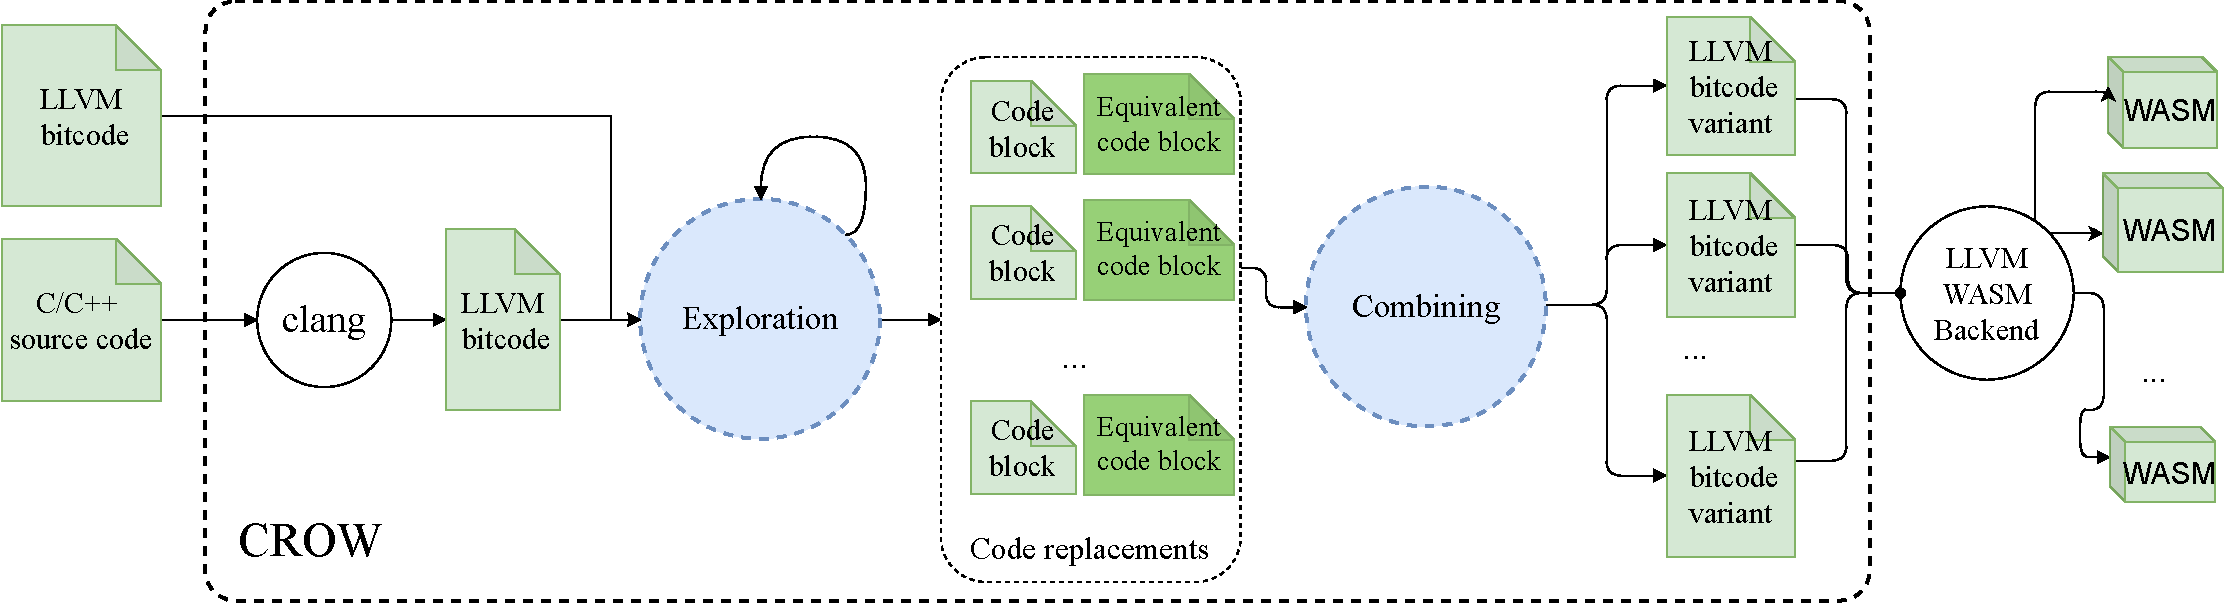
\includegraphics[width=\linewidth]{diagrams/generation/crow.drawio.pdf}
    \caption{CROW workflow to generate program variants. CROW takes C/C++ source codes or LLVM bitcodes to look for code blocks that can be replaced by semantically equivalent code and generates program variants by combining them.}
    \label{diagrams:crow}
\end{figure*}

Figure \ref{diagrams:crow} highlights the main two stages of the CROW's workflow, \textit{exploration} and \textit{combining}. The workflow starts by compiling the input program into the LLVM bitcode using clang from the source code. During the \emph{exploration} stage, CROW takes an LLVM bitcode and, for its code blocks, produces a collection of code replacements that are functionally equivalent to the original program. In the following, we enunciate the definitions we use along with this work for a code block, functional equivalence, and code replacement. 


\begin{definition}{Block (based on Aho \etal \cite{10.5555/6448}):}\label{def:code-block}
    Let $P$ be a program. A block $B$ is a grouping of declarations and statements in $P$ inside a function $F$. 
\end{definition}


\begin{definition}{Functional equivalence modulo program state (based on Le \etal \cite{10.1145/2594291.2594334}):}
    \label{def:functional-equivalence}
    Let $B_1$ and $B_2$ be two code blocks according to \autoref{def:code-block}. We consider the program state before the execution of the block, $S_i$, as the input and the program state after the execution of the block, $S_o$, as the output. $B_1$ and $B_2$ are functionally equivalent if given the same input $S_i$ both codes produce the same output $S_o$.
\end{definition}

\begin{definition}{Code replacement:}
    \label{def:code-replacement}
    Let $P$ be a program and $T$ a pair of code blocks $(B_1, B_2)$. $T$ is a candidate code replacement if $B_1$ and $B_2$ are both functionally equivalent as defined in \autoref{def:functional-equivalence}.
    Applying $T$ to $P$ means replacing $B_1$ by $B_2$. The application of $T$ to $P$ produces a program variant $P'$ which consequently is functionally equivalent to $P$.     
\end{definition}

We implement the \emph{exploration} stage by retargeting a superoptimizer for  LLVM, using its subset of the LLVM intermediate representation. CROW operates at the code block level, taking them from the functions defined inside the input LLVM bitcode module. In addition, the retargeted superoptimizer is in charge of finding the potential places in the original code blocks where a replacement can be applied. Finally, we use the enumerative synthesis strategy of the retargeted superoptimizer to generate code replacements.
The code replacements generated through synthesis are verified, according to \autoref{def:functional-equivalence}, by internally using a theorem prover. 

Moreover, we prevent the superoptimizer from synthesizing instructions that have no correspondence in \wasm for the sake of reducing the searching space for equivalent program variants. Besides, we disable all optimizations in the \wasm LLVM backend that could reverse the superoptimizer transformations, such as constant folding and instructions normalization.

%\todo{We disable cost restrictions and the LLVM backend optimizations...maybe for the assesment RQ ?}

In the \emph{combining} stage, CROW combines the candidate code replacements to generate different LLVM bitcode variants, selecting and merging the code replacements. 
Then for each combination, a variant bitcode is compiled into a \wasm binary if requested. Finally, CROW generates the variants from all possible combinations of code replacements as the power set of all code replacements.  

\end{comment}
\chapter{Methodology} 
\label{chapter:method}

\pagestyle{plain}
% Define some numbers here for the autmation of the tables
\newcommand{\libsodiumfunctions}{869}
\newcommand{\qrcodefunctions}{1849}
\newcommand{\allmewefunctions}{\libsodiumfunctions + \qrcodefunctions}

% Execute a python script for small calculations
\newcommand{\py}[1]{\input{|python3 interpreter.py #1}}
\newcommand{\fromjson}[2]{\input{| jq -r '#2' '#1}}

\newcommand{\corpusrosetta}{Rosetta\xspace}
\newcommand{\corpussodium}{Libsodium\xspace}
\newcommand{\corpusqrcode}{QrCode\xspace}


\newcommand{\DTWStatic}{dt\_static\xspace}
\newcommand{\DTW}{TraceDiff\xspace}
\renewcommand{\tool}{CROW\xspace}

%\todo{Recheck the selection of the modules for sodium}

%This chapter investigates whether we can artificially create program variants through semantically equivalent code transformations. We propose a framework to generate program variants functionally equivalent to their original.
%We introduce the retargeting of a superoptimizer, using its exhaustive search strategy to provide semantically equivalent code transformations. 
%The presented methodology and transformation tool, CROW, are contributions to this thesis.
%We evaluate the usage of CROW on two corpora of open-source and nature diverse programs. 
In this chapter, we present our methodology to answer the research questions enunciated in \autoref{intro:definition:rq}.
We investigate three research questions. In the first question, we aim to investigate the static differences between variants. We evaluate the code properties the lead less or more software diversification.
Our second research question focuses on comparing their behavior during their execution, complementing our first research question. The generated variants should be statically different, but also should provide different observable behavior. 
The final research question evaluates the feasibility of using the program variants in security-sensitive environments. We evaluate our generated program variants in an Edge-Cloud computing platform proposing a novel multivariant execution approach.

% \todo{too generic: READ AGAIN to see how to land this
The main objective of this thesis is to study the feasibility of automatically creating program variants out of preexisting program sources. To achieve this objective,
we use the empirical method \cite{Runeson2020}, proposing a solution and evaluating it through quantitative analyzes in case studies. We follow an iterative and incremental approach on the selection of programs for our corpora. To build our corpora, we find a representative and diverse set of programs to generalize, even when it is unrealistic following an empirical approach, as much as possible our results.
We first enunciate the corpora we share along this work to answer our research questions. Then, we establish the metrics for each research question, set the configuration for the experiments, and describe the protocol.

% Our approach lies under \textit{Design Science} \cite{Runeson2020}, in terms of empirical validation, the scope of the design knowledge gained in a study can be extended by systematically extending the scope of the valudation in subsequent studies. Thus, the size of our corpora can be extended to increase the knowledge of the research area.


\section{Corpora}
\label{section:crow:corpora}

Our experiments assess the impact of artificially created diversity. The first step is to build a suitable corpus of programs' seeds to generate the variants. Then, we answer all our research questions with three corpora which follow two main properties: 1) \emph{functionally diverse:} the selection of the programs is not biased by functionally fixed tasks, for example, the programs in one of our corpora solve from the \textit{Babbage} problem to \textit{Convex Hull} calculation; and 2) \emph{representative:} our corpora have 3021 programs that can be ported to \wasm, representing approximately 40\% of the unique Wasm binaries in the wild \cite{Hilbig2021AnES}.


We build our three corpora in an escalating strategy based on the merging of our previous publications. The first corpus is diverse and contains simple programs in terms of code size, making them easy to manually analyze. The second corpus is a project meant for security-sensitive applications. The third corpus is a QR encoding decoding algorithm. 
%The work of Hilbig \etal \cite{Hilbig2021AnES} shows that approximately 65\% of all \wasm programs come out of C/C++ source code through the LLVM pipeline, and more than 75\% if the Rust language is included. Therefore, all modules in the corpora are considered to come along the LLVM pipeline. 
In the following, we describe the filtering and description of each corpus.

\begin{enumerate}
    \item \textbf{\corpusrosetta}: We take programs from the Rosetta Code project\footnote{\url{http://www.rosettacode.org/wiki/Rosetta_Code}}. This website hosts a curated set of solutions for specific programming tasks in various programming languages. It contains many tasks, from simple ones, such as adding two numbers, to complex algorithms like a compiler lexer. We first collect all C programs from the Rosetta Code, representing $989$ programs as of 01/26/2020. We then apply several filters: the programs should successfully compile and, they should not require user inputs to automatically execute them, the programs should terminate and should not result in non-deterministic results. 
    
    The result of the filtering is a corpus of 303 C programs. All programs include a single function in terms of source code. These programs range from $7$ to $150$ lines of code.

    \item \textbf{\corpussodium}: This project is encryption, decryption, signature, and password hashing library implemented in 102 separated modules. The modules have between $8$ and $2703$ lines of code per function. This project is selected based on two main criteria: first, its importance for security-related applications, and second, its suitability to collect the modules in LLVM intermediate representation. %We select 5 programs that interconnect the 102 modules of the project.

    \item \textbf{\corpusqrcode}: This project is a QrCode and MicroQrCode generator written in Rust. This project contains 2 modules having between $4$ and $725$ lines of code per function. As \corpussodium, we select this project due to its suitability for collecting the modules in their LLVM representation. Remarkably, this project increases the complexity of the previously selected projects due to its integration with the generation of images.
    
\end{enumerate}

In \autoref{table:corpora} we listed the corpus name, the language of the programs in the corpus, the number of modules, the total number of functions, the range of lines of code, and the original location of the corpus. 


%The first corpus, \textbf{CROW prime}, . The second corpus, \textbf{MEWE prime}, is part of the MEWE contribution \cite{}. In \autoref{table:corpora} we summarize the selection criteria, and we mention each corpus properties. With both corpora we evaluate CROW with a total of $303 + \py{\allmewefunctions}$ functions. 

\begin{table}[h]
    \renewcommand{\arraystretch}{1.0}
    \small
    \centering
    \begin{tabular}{l | p{1cm} | l | l | l | p{3.2cm}}
        Corpus & Lang. & No. modules & No. functions & LOC range & Location \\
        \midrule
            % CROW
            \corpusrosetta & C &
            - %\footnote{ The concept of module does not apply for this corpus programs. } 
            &
            303  & 
            7 - 
            150 & 
            \url{https://github.com/KTH/slumps/tree/master/benchmark_programs/rossetta/valid/no_input}\\
        \hline
        \corpussodium & LLVM IR + Rust &
        102 &
        869  &
        8 - 2703 &   
        \url{https://github.com/jedisct1/libsodium/tree/2b5f8f2b6810121c2d9a8cc8a392e01f4d3de433 }\\
        \hline
        \corpusqrcode & LLVM IR + Rust &
        2 &
        1849  & 
        4 - 725   & 
        \url{https://github.com/kennytm/qrcode-rust/commit/faa4397ba7c5f441cb9a2b436c1e84a0d52ae942} \\
        % Total stats
        \hline
        \hline
        \textbf{Total} & & 
        & 
        \py{ 303 + \qrcodefunctions + \libsodiumfunctions} &  
        &     \\

    \end{tabular}
    \caption{Corpora description. The table is composed by the name of the corpus, programming language of the programs in the corpus, the number of modules, the number of functions, the lines of code range and the location of the corpus.}
    \label{table:corpora}
\end{table}


\section{\rqone}
\label{rq1:method}

\begin{figure}[h]
    \centering
    \includegraphics[height=4.1in]{diagrams/RQ1.pdf}
    \caption{The program variants generation for RQ1.}
    \label{diagrams:protocol:rq1}
\end{figure}


This research question investigates whether we can artificially generate program variants for \wasm. We use CROW to generate variants from an original program, written in C/C++ in the case of the \corpusrosetta corpus and LLVM bitcode modules in the case of the \corpussodium and \corpusqrcode. 
In \autoref{diagrams:protocol:rq1} we illustrate the workflow to generate \wasm\ program variants. We pass each function of the corpora to CROW as a program to diversify. To answer RQ1, we study the outcome of this pipeline, the generated \wasm\ variants. 


\subsection*{Metrics}

To assess our approach's ability to generate \wasm\ binaries that are statically different, we compute the number of variants and the number of unique variants for each original function of each corpus. 
On top, we define the aggregation of these former two values to quantitatively evaluate RQ1 at the corpus level. 

We start by defining what a program's population is. This definition can be applied in general to any collection of variants of the same program. All definitions are based upon bytecodes and not the source code of the programs.

\begin{definition}{Program's population $M(P)$:}\label{def:rq1:programspopulation}
    \normalfont 
    Given a program P and its generated variants $v_i$, the program's population is defined as:\\
    $$
        M(P)=\{v_i\ \text{where $v_i$ is a variant of P}\}
    $$

    Notice that the program's population includes the original program P.
\end{definition}

Beyond the program's population, we also want to compare how many program variants are unique. The subset of unique programs in the program's population hints how the variants are different between them and not only against the original program. For example, imagine a program $P$ with two program variants $V_1$ and $V_2$, the program population is composed by $\{P, V_1 \text{ and } V_2\}$, where $V_1$ is different from $P$, and $V_2$ is different from $P$. $V_1$ is either equal or different from $V_2$, the program's population still be the same. If $V_1$ and $V_2$ are equal, then only one unique variant is generated,

%\todo{
%   clarify source code versus byte code for earch definition.

%why are those definitions important? interesting? why do you introduce them?
%}
%Notice that all metrics over programs and their variants make sense only at the population level. Therefore, we compare semantically equivalent programs from the same population.

%\todo{
%   difference unclear or trivial.

%do you need source code versus bytecode?

%clarify
%}

\begin{definition}{Program's unique population $U(P)$:}\label{def:rq1:programsuniquepopulation}
    \normalfont 
    Given a program P and its program's population $M(P)$, the program's unique population is defined as.\\
    $$
        U(P)=\{v\ \in\ M(P)\}
    $$
    such that $\forall v_i,v_j \in U(P)$, $v_i \neg v_j$ $\Rightarrow$ $md5sum(v_i) \ne md5sum(v_j)$.
    $Md5sum(v)$ is the md5 hash calculated over the bytecode stream of the program file $v$. Notice that the original program $P$ is included in $U(P)$.

\end{definition}

\begin{metric}{Program's population size $S(P)$:}\label{metric:rq1:PS}
    \normalfont 
    Given a program P and its program's population $M(P)$ according to \autoref{def:rq1:programspopulation}, the program's population size is defined as.\\
    $$
        S(P)=|M(P)|
    $$
\end{metric}


\begin{metric}{Program's unique population size $US(P)$:}\label{metric:rq1:UP}
    \normalfont 
    Given a program P and its program's unique population $U(P)$ according to \autoref{def:rq1:programsuniquepopulation}, the program's unique population size is defined as.\\
    $$
        US(P)=|U(P)|
    $$
\end{metric}

\newcommand{\corpuspopulationsizename}{Corpus population size\xspace}
\newcommand{\corpusuniquepopulationsizename}{Corpus unique population size\xspace}

\begin{metric}{\corpuspopulationsizename$CS(C)$:}\label{metric:rq1:corpus_pop}
    \normalfont 
    Given a program's corpus $C$, the corpus population size is defined as the sum of all program's population sizes over the corpus $C$:\\
    $$
        CS(C)=\Sigma{S(P)}\ \forall\ P\ \in\ C
    $$
\end{metric}

\begin{metric}{\corpusuniquepopulationsizename$UCS(C)$:}\label{metric:rq1:corpus_pop_unique}
    \normalfont 
    Given a program's corpus $C$, the corpus unique population size is defined as the sum of all program's unique population sizes over the corpus $C$ :\\
    $$
    UCS(C)=\Sigma{US(P)}\ \forall\ P\ \in\ C
    $$
\end{metric}


\subsection*{Protocol}
To generate program variants, we synthesize programs with an enumerative strategy, checking each synthesis for equivalence modulo input \cite{Li2018} against the original program, as it is described in \autoref{section:crow}. For obvious reasons, this space is nearly impossible to explore in a reasonable time as soon as the limit of instructions increases.
Therefore, we use two parameters to control the size of the search space and hence the time required to traverse it.
On the one hand, one can limit the size of the variants. On the other hand, one can limit the set of instructions used for the synthesis. In our experiments for RQ1, we use all instructions in the CROW diversifier synthesis.


The former parameter allows us to find a trade-off between the number of variants that are synthesized and the time taken to produce them. For the current evaluation, given the size of the corpus and the properties of its programs, we set the exploration time to 1 hour maximum per function for \corpusrosetta. In the cases of \corpussodium\ and\ \corpusqrcode, we set the timeout to 5 minutes per function. The decision behind the usage of lower timeout for \corpussodium
and \corpusqrcode is motivated by the properties listed in \autoref{table:corpora}. The latter two corpora are remarkably larger regarding the number of instructions and functions. 

We pass each of the $303 + \libsodiumfunctions + \qrcodefunctions$ functions in the corpora to CROW, as \autoref{diagrams:protocol:rq1} illustrates, to synthesize program variants. We calculate the \emph{Corpus population size} (\autoref{metric:rq1:corpus_pop}) and \emph{Corpus unique population size} (\autoref{metric:rq1:corpus_pop_unique}) for each corpus and conclude by answering RQ1.



\section{\rqtwo}
\label{rq2:method}


\begin{figure*}[h]
    \centering
    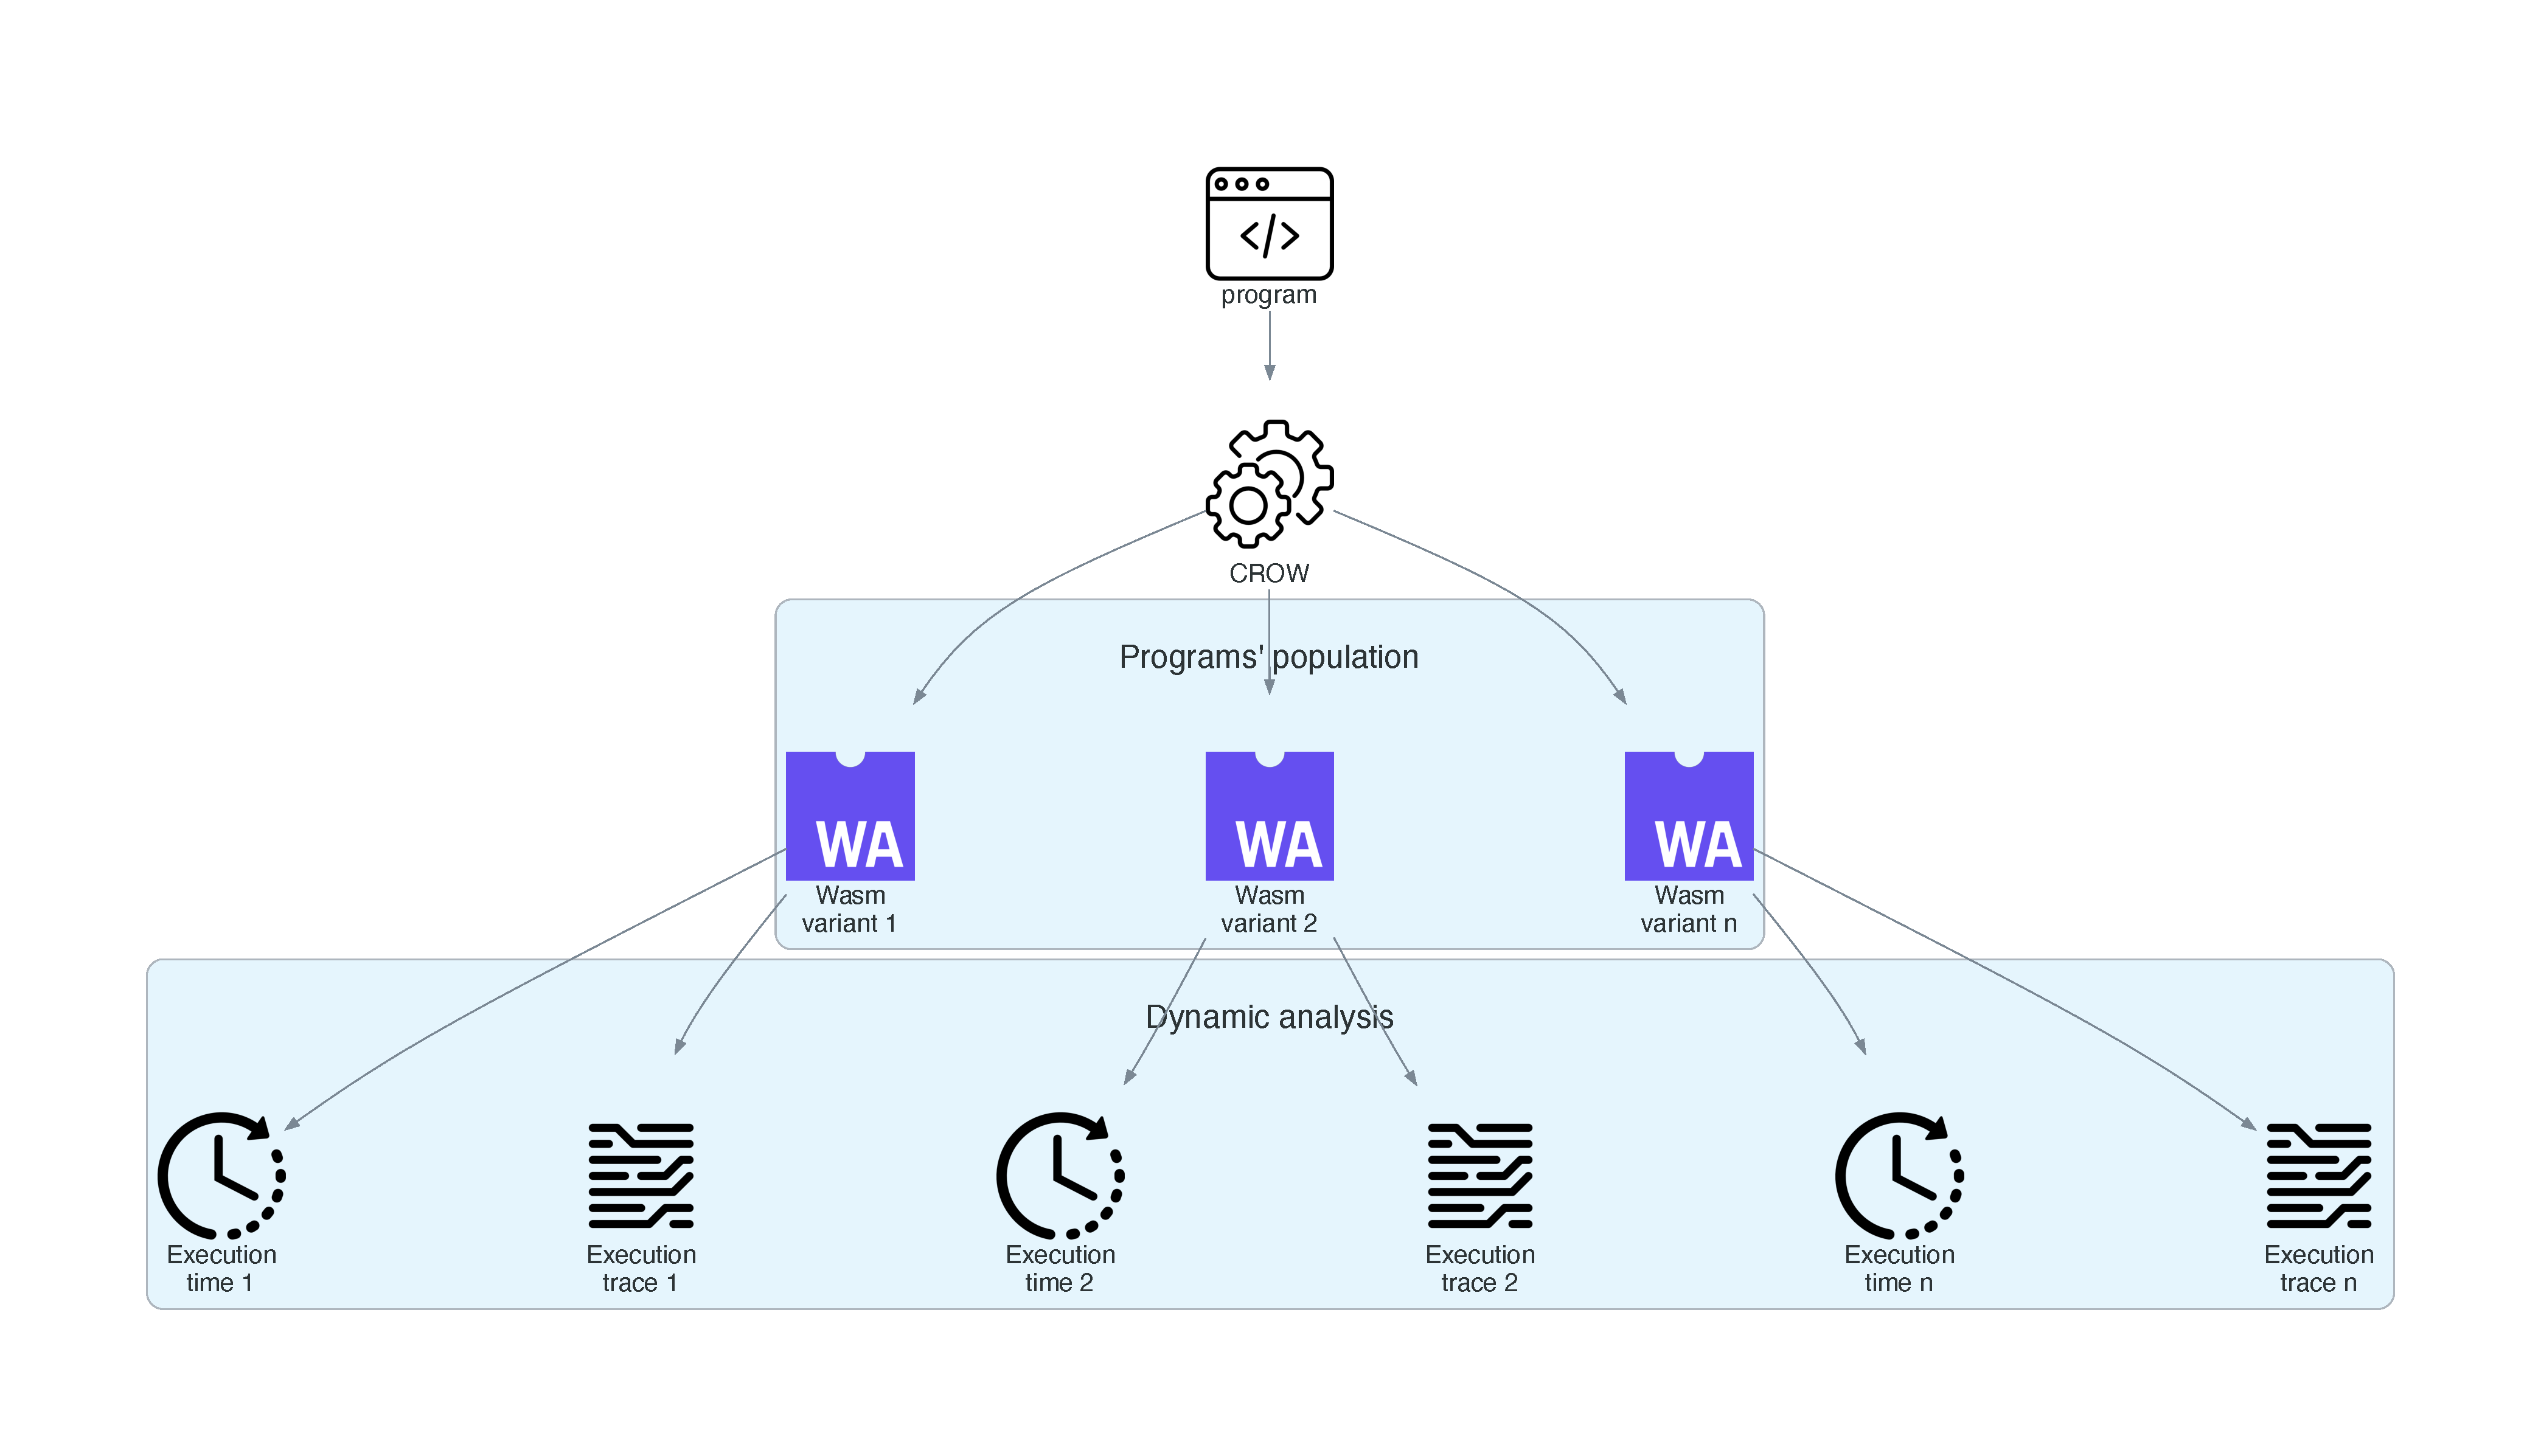
\includegraphics[width=\linewidth]{diagrams/Rq2.pdf}
    \caption{Dynamic analysis for RQ2.}
    \label{diagrams:protocol:rq2}
\end{figure*}

In this second research question, we investigate to what extent the artificially created variants are dynamically different between them and the original program. To conduct this research question, we could separate our experiments into two fields as \autoref{diagrams:protocol:rq2} illustrates: static analysis and dynamic analysis. 
The static analysis focuses on the appreciated differences among the program variants, as well as between the variants and the original program, and we address it in answering RQ1. 
With RQ2, we focus on the last category, the dynamic analysis of the generated variants. This decision is supported because dynamic analysis complements RQ1 and, it is essential to provide a full understanding of diversification.
We use the original functions from \corpusrosetta corpus described in \autoref{section:crow:corpora} and their variants generated to answer RQ1. 
We use only \corpusrosetta to answer RQ2 because this corpus is composed of simple programs that can be executed directly without user interaction, \ie we only need to call the interpreter passing the \wasm binary to it. 

\todo{Motivate, Increasing attack surface does not necesarilly has an impact on defence. For example, reordering instructions for code blocks that are never executed does not impact attacker}

To dynamically compare programs and their variants, we execute each program on each programs' population to collect and execution times. We define execution trace and execution time in the following section.
%\todo{vague and subjective, avoid or elaborate: We perform fine-grained} comparisons by comparing the traces and execution times for all pairs of programs. Therefore, the defined metrics are formulated to support a pairwise comparison strategy.
%In the following, we define the metrics used to answer RQ2.

\subsection*{Metrics}
\label{rq2:metrics}

We compare the execution traces of two any programs of the same population with a global alignment metric. We propose a global alignment approach using Dynamic Time Warping (DTW).
Dynamic Time Warping \cite{NEEDLEMAN1970443} computes the global alignment between two sequences. It returns a value capturing the cost of this alignment, which is a distance metric. The larger the DTW distance, the more different the two sequences are.
DTW has been used for comparing traces in different domains. For software, De A. Maia \etal \cite{ Maia08usinga} proposed to identify similarity between programs from execution traces.
In our experiments, we define the traces as the sequence of the stack operations during runtime, \ie the consecutive list of \texttt{push} and \texttt{pop} operations performed by the \wasm engine during the execution of the program.
In the following, we define the $\DTW$ metric. 
 


\todo{before, define this and give an illutrative listing plus, says how you collect those traces, that's part of the protocol: between the stack operation traces }

\begin{metric}{\DTW{}:}
\label{metric:stack}
\normalfont 
	Given two programs P and P' from the same program's population, \DTW{}(P,P'), computes the DTW distance collected during their execution. \\
	A \DTW{} of $0$ means that both traces are identical.
	The higher the value, the more different the traces. 
\end{metric}



Moreover, we use the execution time distribution of the programs in the population to complement the answer to RQ2. For each program pair in the programs' population, we compare their execution time distributions. We define the execution time as follows:

\begin{metric}{Execution time:}\label{metric:time}
    \normalfont 
	Given a \wasm program P, the execution time is the time spent to execute the binary.
\end{metric}



%\subsection{Variants preservation}

\subsection*{Protocol}

% Dynamic
To compare program and variants behavior during runtime, we analyze all the unique program variants generated to answer RQ1 in a pairwise comparison using the value of aligning their execution traces (\autoref{metric:stack}). We use SWAM\footnote{\url{https://github.com/satabin/swam}} to execute each program and variant to collect the stack operation traces. SWAM is a \wasm interpreter that provides functionalities to capture the dynamic information of \wasm program executions, including the virtual stack operations.
% \todo{Can the reader runderstand that? We want to remark that we only collect the stack operation traces due to the memory-agnosticism of our approach to generate variants. Our approach does not change the memory-like operations of the original code.}

Furthermore, we collect the execution time, \autoref{metric:time}, for all programs and their variants. We compare the collected execution time distributions between programs using a Mann-Withney U test \cite{mann1947} in a pairwise strategy.

%\todo{Maybe the first time that Mann-Withney is mentioned I should describe what it is}

 


\section{\rqthree}
\label{rq3:method}


\todo{The last method is too short}


\newcommand{\mewe}{MEWE\xspace}

\begin{figure}[h]
    \centering
    \includegraphics[width=0.8\linewidth]{diagrams/Rq3.pdf}
    \caption{Multivariant binary creation and workflow for RQ3 answering.}
    \label{diagrams:protocol:rq3}
\end{figure}

In the last research question, we study whether the created variants can be used in real-world applications and what properties offer the composition of the variants as multivariant binaries. \todo{Not defined: We build multivariant binaries}, and we deploy and execute them at the Edge. The process of \emph{mixing} multiple variants into one multivariant binary is an essential contribution of the thesis that is presented in details in \cite{2021arXiv210808125C}. RQ3 focuses on analyzing the impact of this contribution on execution times. To answer RQ3, we use the variants generated for the programs of \corpussodium and \corpusqrcode corpora, we take $2 + 5$ programs interconnecting the LLVM bitcode modules (mentioned in \autoref{table:corpora}). We illustrate the protocol to answer RQ3 in \autoref{diagrams:protocol:rq3} starting from the creation of the programs' population.



%The workflow starts by using the programs' population of each program generated in RQ1 to create the multivariant binaries. We deploy the multivariant binaries at the Edge, and we collect their execution times. We measure the differences for the execution times on the edge. Then, we discuss how multivariant binaries contribute to less predictable timing side-channels.

\subsection*{Metrics}

We use the execution time of the multivariant binaries to answer RQ3. We use the same metric defined in \autoref{metric:time} for the execution time of multivariant binaries.

\subsection*{Protocol}


We run the experiments to answer RQ3 on the Edge, \todo{too fast. tell the reader why you need HTTP now: executing the multivariant binaries as end-to-end HTTP services.} 
The execution times are measured at the backend space, \ie we collect the execution times inside the Edge node and not from the client computer. Therefore, we instrument the binaries to return the execution time as an HTTP header. We do this process for the original program and its multivariant binary. We deploy and execute the original and the multivariant binaries on 64 edge nodes located around the world \todo{Add illustrative map}.


We collect 100k execution times for each binary \todo{Why? Cite blackhat paper and the need of 1 million traces multiplied by the number of nodes}, both the original and multivariant binaries.
We perform a Mann-Withney U test \cite{mann1947} to compare both execution time distributions. 
If the P-value is lower than 0.05, the two compared distributions are different.

%\pagebreak

\section*{Conclusions}

This chapter presents the methodology we follow to answer our three research questions. We first describe and propose the corpora of programs used in this work. We propose to measure the ability of our approach to generate variants out of \py{303  + \libsodiumfunctions + \qrcodefunctions} functions of our corpora. Then, we suggest using the generated variants to study to what extent they offer different observable behavior through dynamic analysis. We propose a protocol to study the impact of the composition variants in a multivariant binary deployed at the Edge. Besides, we enumerate and enunciate the properties and metrics that might lead us to answer the impact of automatic diversification for \wasm programs. In the next chapter, we present and discuss the results obtained with this methodology.


%\todo{Add the unique and the total.}
%\todo{Change metrics and the name of dt\_dyn.}
%\todo{Remove growing factor.}
%\todo{Explain what a quantile-quantile plot is.}

\clearpage
\chapter{Methodology} 
\label{chapter:method}

\pagestyle{plain}
% Define some numbers here for the autmation of the tables
\newcommand{\libsodiumfunctions}{869}
\newcommand{\qrcodefunctions}{1849}
\newcommand{\allmewefunctions}{\libsodiumfunctions + \qrcodefunctions}

% Execute a python script for small calculations
\newcommand{\py}[1]{\input{|python3 interpreter.py #1}}
\newcommand{\fromjson}[2]{\input{| jq -r '#2' '#1}}

\newcommand{\corpusrosetta}{Rosetta\xspace}
\newcommand{\corpussodium}{Libsodium\xspace}
\newcommand{\corpusqrcode}{QrCode\xspace}


\newcommand{\DTWStatic}{dt\_static\xspace}
\newcommand{\DTW}{TraceDiff\xspace}
\renewcommand{\tool}{CROW\xspace}

%\todo{Recheck the selection of the modules for sodium}

%This chapter investigates whether we can artificially create program variants through semantically equivalent code transformations. We propose a framework to generate program variants functionally equivalent to their original.
%We introduce the retargeting of a superoptimizer, using its exhaustive search strategy to provide semantically equivalent code transformations. 
%The presented methodology and transformation tool, CROW, are contributions to this thesis.
%We evaluate the usage of CROW on two corpora of open-source and nature diverse programs. 
In this chapter, we present our methodology to answer the research questions enunciated in \autoref{intro:definition:rq}.
We investigate three research questions. In the first question, we aim to investigate the static differences between variants. We evaluate the code properties the lead less or more software diversification.
Our second research question focuses on comparing their behavior during their execution, complementing our first research question. The generated variants should be statically different, but also should provide different observable behavior. 
The final research question evaluates the feasibility of using the program variants in security-sensitive environments. We evaluate our generated program variants in an Edge-Cloud computing platform proposing a novel multivariant execution approach.

% \todo{too generic: READ AGAIN to see how to land this
The main objective of this thesis is to study the feasibility of automatically creating program variants out of preexisting program sources. To achieve this objective,
we use the empirical method \cite{Runeson2020}, proposing a solution and evaluating it through quantitative analyzes in case studies. We follow an iterative and incremental approach on the selection of programs for our corpora. To build our corpora, we find a representative and diverse set of programs to generalize, even when it is unrealistic following an empirical approach, as much as possible our results.
We first enunciate the corpora we share along this work to answer our research questions. Then, we establish the metrics for each research question, set the configuration for the experiments, and describe the protocol.

% Our approach lies under \textit{Design Science} \cite{Runeson2020}, in terms of empirical validation, the scope of the design knowledge gained in a study can be extended by systematically extending the scope of the valudation in subsequent studies. Thus, the size of our corpora can be extended to increase the knowledge of the research area.


\section{Corpora}
\label{section:crow:corpora}

Our experiments assess the impact of artificially created diversity. The first step is to build a suitable corpus of programs' seeds to generate the variants. Then, we answer all our research questions with three corpora which follow two main properties: 1) \emph{functionally diverse:} the selection of the programs is not biased by functionally fixed tasks, for example, the programs in one of our corpora solve from the \textit{Babbage} problem to \textit{Convex Hull} calculation; and 2) \emph{representative:} our corpora have 3021 programs that can be ported to \wasm, representing approximately 40\% of the unique Wasm binaries in the wild \cite{Hilbig2021AnES}.


We build our three corpora in an escalating strategy based on the merging of our previous publications. The first corpus is diverse and contains simple programs in terms of code size, making them easy to manually analyze. The second corpus is a project meant for security-sensitive applications. The third corpus is a QR encoding decoding algorithm. 
%The work of Hilbig \etal \cite{Hilbig2021AnES} shows that approximately 65\% of all \wasm programs come out of C/C++ source code through the LLVM pipeline, and more than 75\% if the Rust language is included. Therefore, all modules in the corpora are considered to come along the LLVM pipeline. 
In the following, we describe the filtering and description of each corpus.

\begin{enumerate}
    \item \textbf{\corpusrosetta}: We take programs from the Rosetta Code project\footnote{\url{http://www.rosettacode.org/wiki/Rosetta_Code}}. This website hosts a curated set of solutions for specific programming tasks in various programming languages. It contains many tasks, from simple ones, such as adding two numbers, to complex algorithms like a compiler lexer. We first collect all C programs from the Rosetta Code, representing $989$ programs as of 01/26/2020. We then apply several filters: the programs should successfully compile and, they should not require user inputs to automatically execute them, the programs should terminate and should not result in non-deterministic results. 
    
    The result of the filtering is a corpus of 303 C programs. All programs include a single function in terms of source code. These programs range from $7$ to $150$ lines of code.

    \item \textbf{\corpussodium}: This project is encryption, decryption, signature, and password hashing library implemented in 102 separated modules. The modules have between $8$ and $2703$ lines of code per function. This project is selected based on two main criteria: first, its importance for security-related applications, and second, its suitability to collect the modules in LLVM intermediate representation. %We select 5 programs that interconnect the 102 modules of the project.

    \item \textbf{\corpusqrcode}: This project is a QrCode and MicroQrCode generator written in Rust. This project contains 2 modules having between $4$ and $725$ lines of code per function. As \corpussodium, we select this project due to its suitability for collecting the modules in their LLVM representation. Remarkably, this project increases the complexity of the previously selected projects due to its integration with the generation of images.
    
\end{enumerate}

In \autoref{table:corpora} we listed the corpus name, the language of the programs in the corpus, the number of modules, the total number of functions, the range of lines of code, and the original location of the corpus. 


%The first corpus, \textbf{CROW prime}, . The second corpus, \textbf{MEWE prime}, is part of the MEWE contribution \cite{}. In \autoref{table:corpora} we summarize the selection criteria, and we mention each corpus properties. With both corpora we evaluate CROW with a total of $303 + \py{\allmewefunctions}$ functions. 

\begin{table}[h]
    \renewcommand{\arraystretch}{1.0}
    \small
    \centering
    \begin{tabular}{l | p{1cm} | l | l | l | p{3.2cm}}
        Corpus & Lang. & No. modules & No. functions & LOC range & Location \\
        \midrule
            % CROW
            \corpusrosetta & C &
            - %\footnote{ The concept of module does not apply for this corpus programs. } 
            &
            303  & 
            7 - 
            150 & 
            \url{https://github.com/KTH/slumps/tree/master/benchmark_programs/rossetta/valid/no_input}\\
        \hline
        \corpussodium & LLVM IR + Rust &
        102 &
        869  &
        8 - 2703 &   
        \url{https://github.com/jedisct1/libsodium/tree/2b5f8f2b6810121c2d9a8cc8a392e01f4d3de433 }\\
        \hline
        \corpusqrcode & LLVM IR + Rust &
        2 &
        1849  & 
        4 - 725   & 
        \url{https://github.com/kennytm/qrcode-rust/commit/faa4397ba7c5f441cb9a2b436c1e84a0d52ae942} \\
        % Total stats
        \hline
        \hline
        \textbf{Total} & & 
        & 
        \py{ 303 + \qrcodefunctions + \libsodiumfunctions} &  
        &     \\

    \end{tabular}
    \caption{Corpora description. The table is composed by the name of the corpus, programming language of the programs in the corpus, the number of modules, the number of functions, the lines of code range and the location of the corpus.}
    \label{table:corpora}
\end{table}


\section{\rqone}
\label{rq1:method}

\begin{figure}[h]
    \centering
    \includegraphics[height=4.1in]{diagrams/RQ1.pdf}
    \caption{The program variants generation for RQ1.}
    \label{diagrams:protocol:rq1}
\end{figure}


This research question investigates whether we can artificially generate program variants for \wasm. We use CROW to generate variants from an original program, written in C/C++ in the case of the \corpusrosetta corpus and LLVM bitcode modules in the case of the \corpussodium and \corpusqrcode. 
In \autoref{diagrams:protocol:rq1} we illustrate the workflow to generate \wasm\ program variants. We pass each function of the corpora to CROW as a program to diversify. To answer RQ1, we study the outcome of this pipeline, the generated \wasm\ variants. 


\subsection*{Metrics}

To assess our approach's ability to generate \wasm\ binaries that are statically different, we compute the number of variants and the number of unique variants for each original function of each corpus. 
On top, we define the aggregation of these former two values to quantitatively evaluate RQ1 at the corpus level. 

We start by defining what a program's population is. This definition can be applied in general to any collection of variants of the same program. All definitions are based upon bytecodes and not the source code of the programs.

\begin{definition}{Program's population $M(P)$:}\label{def:rq1:programspopulation}
    \normalfont 
    Given a program P and its generated variants $v_i$, the program's population is defined as:\\
    $$
        M(P)=\{v_i\ \text{where $v_i$ is a variant of P}\}
    $$

    Notice that the program's population includes the original program P.
\end{definition}

Beyond the program's population, we also want to compare how many program variants are unique. The subset of unique programs in the program's population hints how the variants are different between them and not only against the original program. For example, imagine a program $P$ with two program variants $V_1$ and $V_2$, the program population is composed by $\{P, V_1 \text{ and } V_2\}$, where $V_1$ is different from $P$, and $V_2$ is different from $P$. $V_1$ is either equal or different from $V_2$, the program's population still be the same. If $V_1$ and $V_2$ are equal, then only one unique variant is generated,

%\todo{
%   clarify source code versus byte code for earch definition.

%why are those definitions important? interesting? why do you introduce them?
%}
%Notice that all metrics over programs and their variants make sense only at the population level. Therefore, we compare semantically equivalent programs from the same population.

%\todo{
%   difference unclear or trivial.

%do you need source code versus bytecode?

%clarify
%}

\begin{definition}{Program's unique population $U(P)$:}\label{def:rq1:programsuniquepopulation}
    \normalfont 
    Given a program P and its program's population $M(P)$, the program's unique population is defined as.\\
    $$
        U(P)=\{v\ \in\ M(P)\}
    $$
    such that $\forall v_i,v_j \in U(P)$, $v_i \neg v_j$ $\Rightarrow$ $md5sum(v_i) \ne md5sum(v_j)$.
    $Md5sum(v)$ is the md5 hash calculated over the bytecode stream of the program file $v$. Notice that the original program $P$ is included in $U(P)$.

\end{definition}

\begin{metric}{Program's population size $S(P)$:}\label{metric:rq1:PS}
    \normalfont 
    Given a program P and its program's population $M(P)$ according to \autoref{def:rq1:programspopulation}, the program's population size is defined as.\\
    $$
        S(P)=|M(P)|
    $$
\end{metric}


\begin{metric}{Program's unique population size $US(P)$:}\label{metric:rq1:UP}
    \normalfont 
    Given a program P and its program's unique population $U(P)$ according to \autoref{def:rq1:programsuniquepopulation}, the program's unique population size is defined as.\\
    $$
        US(P)=|U(P)|
    $$
\end{metric}

\newcommand{\corpuspopulationsizename}{Corpus population size\xspace}
\newcommand{\corpusuniquepopulationsizename}{Corpus unique population size\xspace}

\begin{metric}{\corpuspopulationsizename$CS(C)$:}\label{metric:rq1:corpus_pop}
    \normalfont 
    Given a program's corpus $C$, the corpus population size is defined as the sum of all program's population sizes over the corpus $C$:\\
    $$
        CS(C)=\Sigma{S(P)}\ \forall\ P\ \in\ C
    $$
\end{metric}

\begin{metric}{\corpusuniquepopulationsizename$UCS(C)$:}\label{metric:rq1:corpus_pop_unique}
    \normalfont 
    Given a program's corpus $C$, the corpus unique population size is defined as the sum of all program's unique population sizes over the corpus $C$ :\\
    $$
    UCS(C)=\Sigma{US(P)}\ \forall\ P\ \in\ C
    $$
\end{metric}


\subsection*{Protocol}
To generate program variants, we synthesize programs with an enumerative strategy, checking each synthesis for equivalence modulo input \cite{Li2018} against the original program, as it is described in \autoref{section:crow}. For obvious reasons, this space is nearly impossible to explore in a reasonable time as soon as the limit of instructions increases.
Therefore, we use two parameters to control the size of the search space and hence the time required to traverse it.
On the one hand, one can limit the size of the variants. On the other hand, one can limit the set of instructions used for the synthesis. In our experiments for RQ1, we use all instructions in the CROW diversifier synthesis.


The former parameter allows us to find a trade-off between the number of variants that are synthesized and the time taken to produce them. For the current evaluation, given the size of the corpus and the properties of its programs, we set the exploration time to 1 hour maximum per function for \corpusrosetta. In the cases of \corpussodium\ and\ \corpusqrcode, we set the timeout to 5 minutes per function. The decision behind the usage of lower timeout for \corpussodium
and \corpusqrcode is motivated by the properties listed in \autoref{table:corpora}. The latter two corpora are remarkably larger regarding the number of instructions and functions. 

We pass each of the $303 + \libsodiumfunctions + \qrcodefunctions$ functions in the corpora to CROW, as \autoref{diagrams:protocol:rq1} illustrates, to synthesize program variants. We calculate the \emph{Corpus population size} (\autoref{metric:rq1:corpus_pop}) and \emph{Corpus unique population size} (\autoref{metric:rq1:corpus_pop_unique}) for each corpus and conclude by answering RQ1.



\section{\rqtwo}
\label{rq2:method}


\begin{figure*}[h]
    \centering
    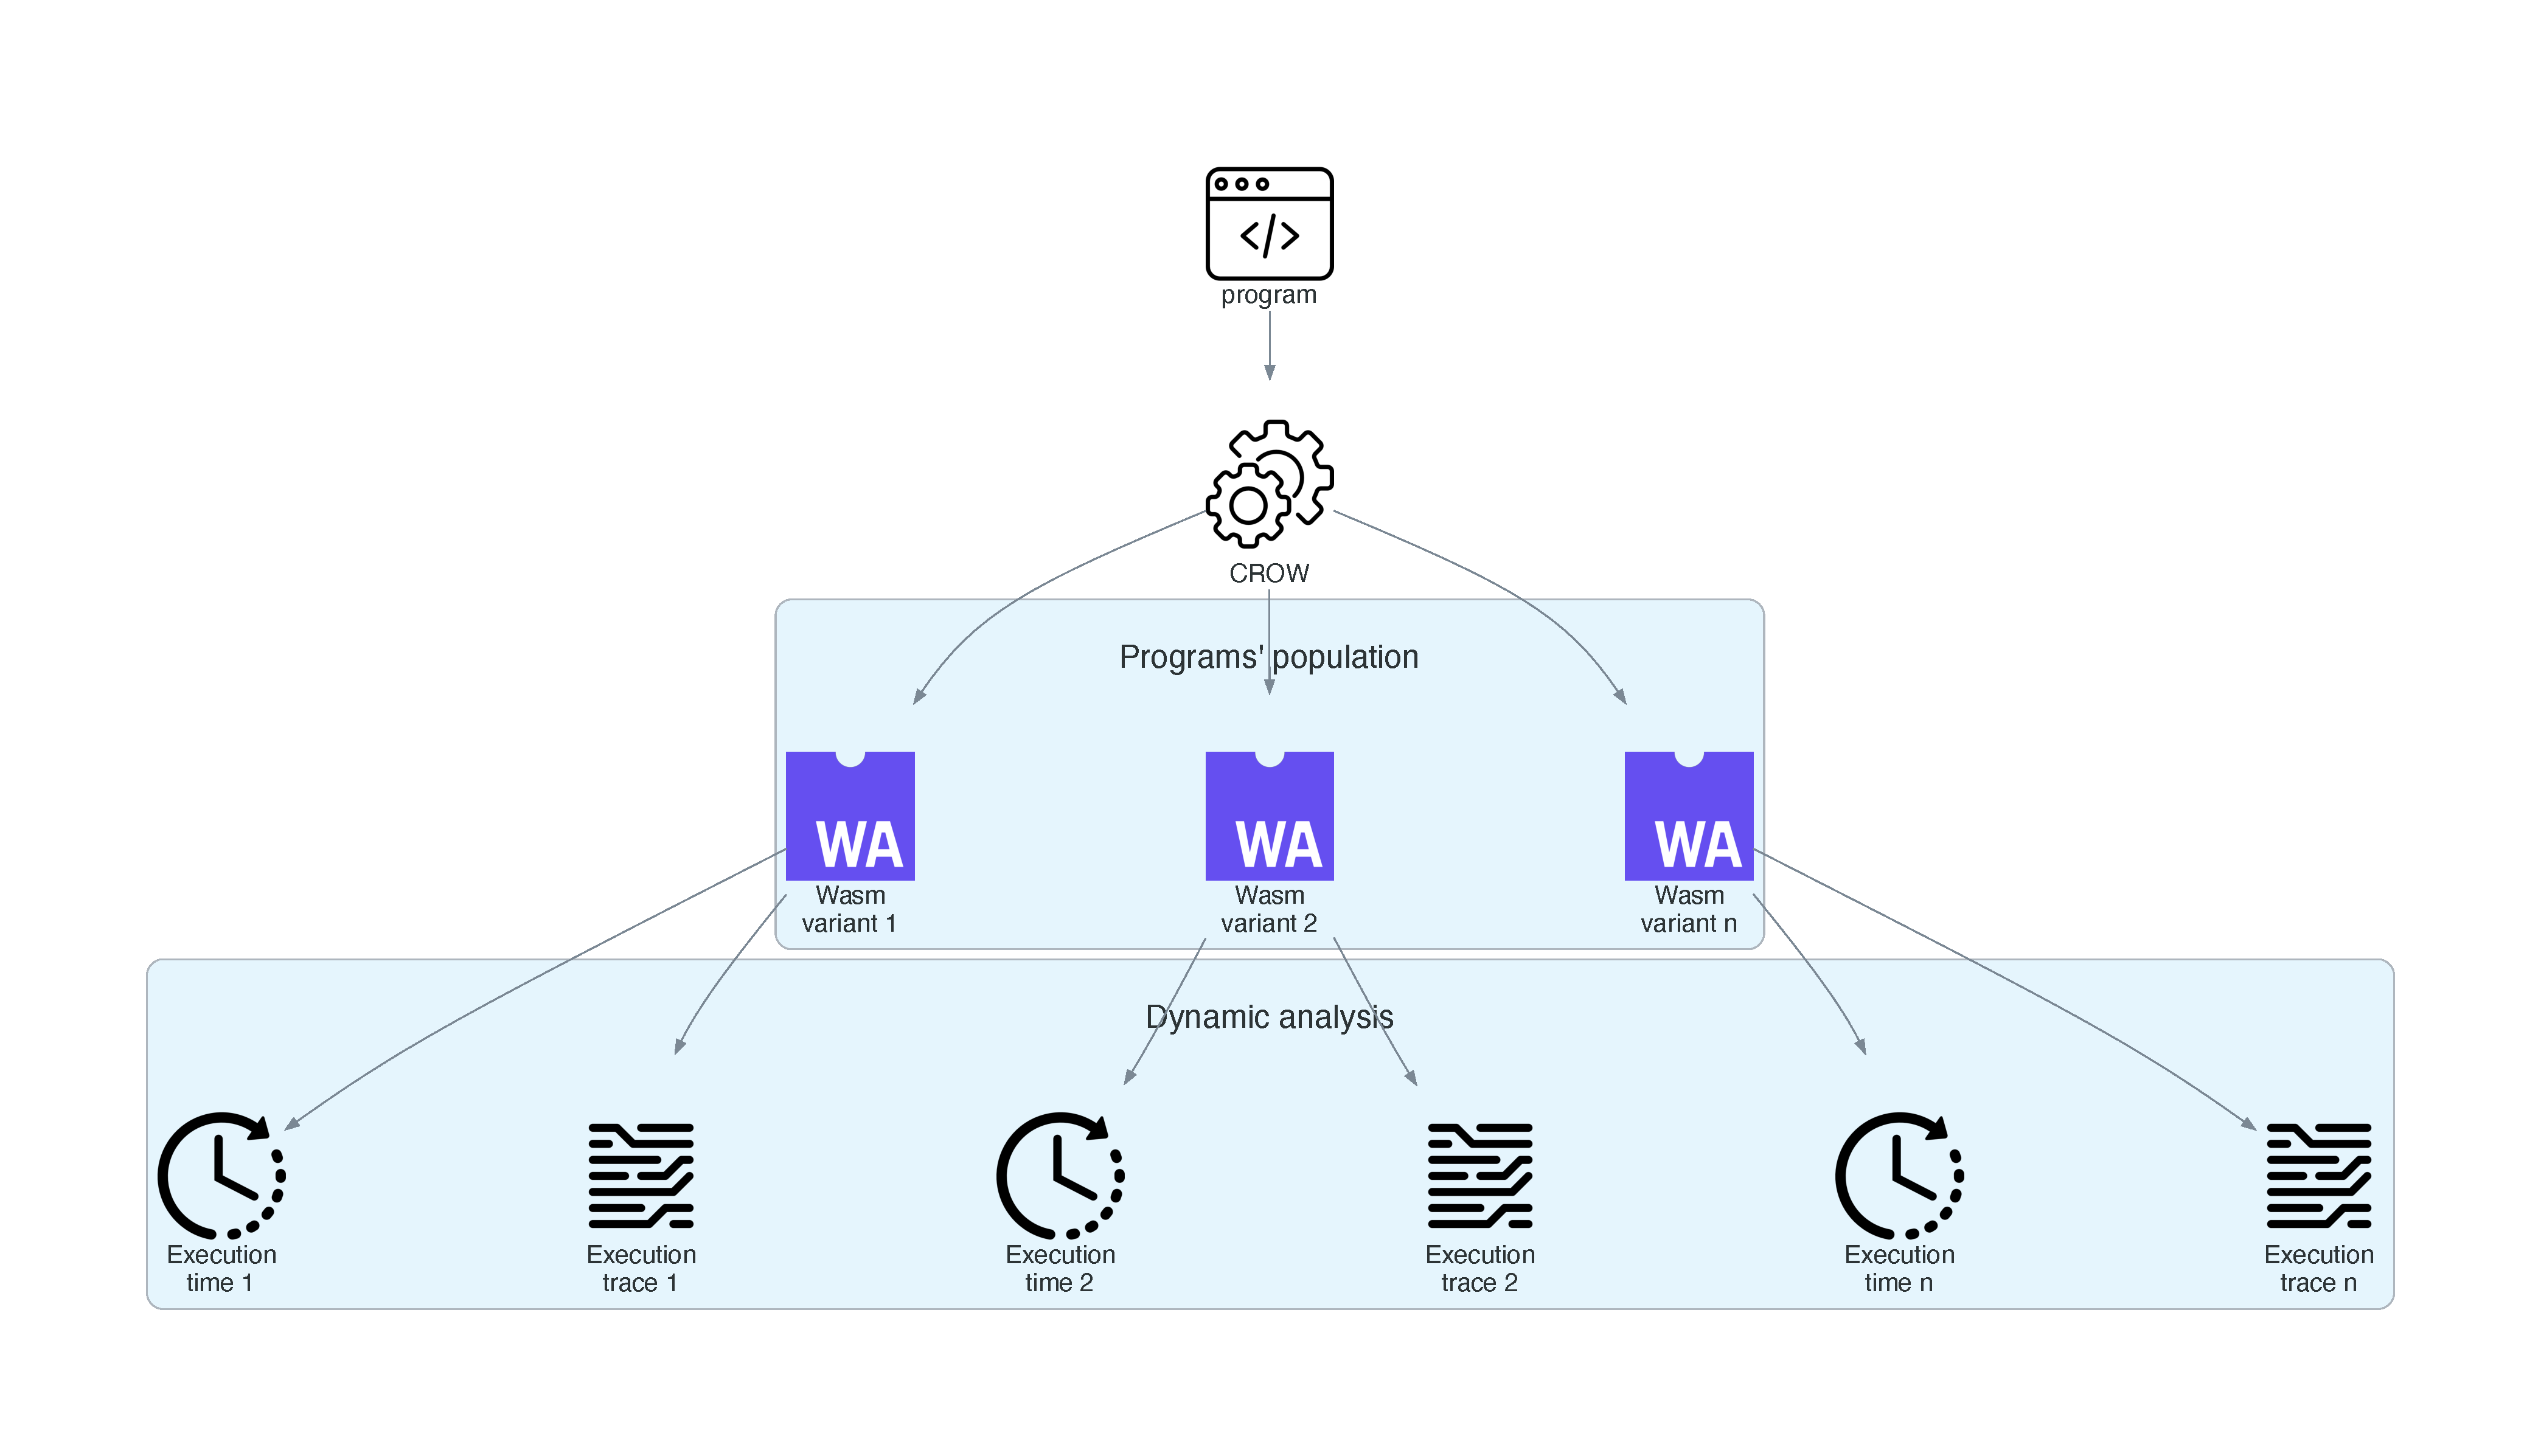
\includegraphics[width=\linewidth]{diagrams/Rq2.pdf}
    \caption{Dynamic analysis for RQ2.}
    \label{diagrams:protocol:rq2}
\end{figure*}

In this second research question, we investigate to what extent the artificially created variants are dynamically different between them and the original program. To conduct this research question, we could separate our experiments into two fields as \autoref{diagrams:protocol:rq2} illustrates: static analysis and dynamic analysis. 
The static analysis focuses on the appreciated differences among the program variants, as well as between the variants and the original program, and we address it in answering RQ1. 
With RQ2, we focus on the last category, the dynamic analysis of the generated variants. This decision is supported because dynamic analysis complements RQ1 and, it is essential to provide a full understanding of diversification.
We use the original functions from \corpusrosetta corpus described in \autoref{section:crow:corpora} and their variants generated to answer RQ1. 
We use only \corpusrosetta to answer RQ2 because this corpus is composed of simple programs that can be executed directly without user interaction, \ie we only need to call the interpreter passing the \wasm binary to it. 

\todo{Motivate, Increasing attack surface does not necesarilly has an impact on defence. For example, reordering instructions for code blocks that are never executed does not impact attacker}

To dynamically compare programs and their variants, we execute each program on each programs' population to collect and execution times. We define execution trace and execution time in the following section.
%\todo{vague and subjective, avoid or elaborate: We perform fine-grained} comparisons by comparing the traces and execution times for all pairs of programs. Therefore, the defined metrics are formulated to support a pairwise comparison strategy.
%In the following, we define the metrics used to answer RQ2.

\subsection*{Metrics}
\label{rq2:metrics}

We compare the execution traces of two any programs of the same population with a global alignment metric. We propose a global alignment approach using Dynamic Time Warping (DTW).
Dynamic Time Warping \cite{NEEDLEMAN1970443} computes the global alignment between two sequences. It returns a value capturing the cost of this alignment, which is a distance metric. The larger the DTW distance, the more different the two sequences are.
DTW has been used for comparing traces in different domains. For software, De A. Maia \etal \cite{ Maia08usinga} proposed to identify similarity between programs from execution traces.
In our experiments, we define the traces as the sequence of the stack operations during runtime, \ie the consecutive list of \texttt{push} and \texttt{pop} operations performed by the \wasm engine during the execution of the program.
In the following, we define the $\DTW$ metric. 
 


\todo{before, define this and give an illutrative listing plus, says how you collect those traces, that's part of the protocol: between the stack operation traces }

\begin{metric}{\DTW{}:}
\label{metric:stack}
\normalfont 
	Given two programs P and P' from the same program's population, \DTW{}(P,P'), computes the DTW distance collected during their execution. \\
	A \DTW{} of $0$ means that both traces are identical.
	The higher the value, the more different the traces. 
\end{metric}



Moreover, we use the execution time distribution of the programs in the population to complement the answer to RQ2. For each program pair in the programs' population, we compare their execution time distributions. We define the execution time as follows:

\begin{metric}{Execution time:}\label{metric:time}
    \normalfont 
	Given a \wasm program P, the execution time is the time spent to execute the binary.
\end{metric}



%\subsection{Variants preservation}

\subsection*{Protocol}

% Dynamic
To compare program and variants behavior during runtime, we analyze all the unique program variants generated to answer RQ1 in a pairwise comparison using the value of aligning their execution traces (\autoref{metric:stack}). We use SWAM\footnote{\url{https://github.com/satabin/swam}} to execute each program and variant to collect the stack operation traces. SWAM is a \wasm interpreter that provides functionalities to capture the dynamic information of \wasm program executions, including the virtual stack operations.
% \todo{Can the reader runderstand that? We want to remark that we only collect the stack operation traces due to the memory-agnosticism of our approach to generate variants. Our approach does not change the memory-like operations of the original code.}

Furthermore, we collect the execution time, \autoref{metric:time}, for all programs and their variants. We compare the collected execution time distributions between programs using a Mann-Withney U test \cite{mann1947} in a pairwise strategy.

%\todo{Maybe the first time that Mann-Withney is mentioned I should describe what it is}

 


\section{\rqthree}
\label{rq3:method}


\todo{The last method is too short}


\newcommand{\mewe}{MEWE\xspace}

\begin{figure}[h]
    \centering
    \includegraphics[width=0.8\linewidth]{diagrams/Rq3.pdf}
    \caption{Multivariant binary creation and workflow for RQ3 answering.}
    \label{diagrams:protocol:rq3}
\end{figure}

In the last research question, we study whether the created variants can be used in real-world applications and what properties offer the composition of the variants as multivariant binaries. \todo{Not defined: We build multivariant binaries}, and we deploy and execute them at the Edge. The process of \emph{mixing} multiple variants into one multivariant binary is an essential contribution of the thesis that is presented in details in \cite{2021arXiv210808125C}. RQ3 focuses on analyzing the impact of this contribution on execution times. To answer RQ3, we use the variants generated for the programs of \corpussodium and \corpusqrcode corpora, we take $2 + 5$ programs interconnecting the LLVM bitcode modules (mentioned in \autoref{table:corpora}). We illustrate the protocol to answer RQ3 in \autoref{diagrams:protocol:rq3} starting from the creation of the programs' population.



%The workflow starts by using the programs' population of each program generated in RQ1 to create the multivariant binaries. We deploy the multivariant binaries at the Edge, and we collect their execution times. We measure the differences for the execution times on the edge. Then, we discuss how multivariant binaries contribute to less predictable timing side-channels.

\subsection*{Metrics}

We use the execution time of the multivariant binaries to answer RQ3. We use the same metric defined in \autoref{metric:time} for the execution time of multivariant binaries.

\subsection*{Protocol}


We run the experiments to answer RQ3 on the Edge, \todo{too fast. tell the reader why you need HTTP now: executing the multivariant binaries as end-to-end HTTP services.} 
The execution times are measured at the backend space, \ie we collect the execution times inside the Edge node and not from the client computer. Therefore, we instrument the binaries to return the execution time as an HTTP header. We do this process for the original program and its multivariant binary. We deploy and execute the original and the multivariant binaries on 64 edge nodes located around the world \todo{Add illustrative map}.


We collect 100k execution times for each binary \todo{Why? Cite blackhat paper and the need of 1 million traces multiplied by the number of nodes}, both the original and multivariant binaries.
We perform a Mann-Withney U test \cite{mann1947} to compare both execution time distributions. 
If the P-value is lower than 0.05, the two compared distributions are different.

%\pagebreak

\section*{Conclusions}

This chapter presents the methodology we follow to answer our three research questions. We first describe and propose the corpora of programs used in this work. We propose to measure the ability of our approach to generate variants out of \py{303  + \libsodiumfunctions + \qrcodefunctions} functions of our corpora. Then, we suggest using the generated variants to study to what extent they offer different observable behavior through dynamic analysis. We propose a protocol to study the impact of the composition variants in a multivariant binary deployed at the Edge. Besides, we enumerate and enunciate the properties and metrics that might lead us to answer the impact of automatic diversification for \wasm programs. In the next chapter, we present and discuss the results obtained with this methodology.


%\todo{Add the unique and the total.}
%\todo{Change metrics and the name of dt\_dyn.}
%\todo{Remove growing factor.}
%\todo{Explain what a quantile-quantile plot is.}

\clearpage
\chapter{Conclusions}

%\Chapter{Variant's application}{RQ3. To what extent the generated variants can be used in security vulnerable applications?} 

%\section{Security MTD}

%\section{Reliability (CVE + fuzz) future work}
\chapter{Conclusion and Future Work}
\label{chapter:conclude}

\wasm\ has become a new technology for web browsers and standalone engines such as the ones used in edge-cloud platforms. \wasm\ is designed with security and sandboxing premises, yet, is still vulnerable.
Besides, since it is a relatively new technology, new vulnerabilities appear in the wild faster than the adoption of patches and defenses.
As a widely studied field, software diversification could be a solution for known and yet-unknown vulnerabilities. Yet, there is no research on this field for \wasm.

We propose an automatic approach to generate software diversification for \wasm\ in this work. 
In addition, we provide complementary implementation for our approaches, including a generic LLVM superdiversifier that potentially extends our ideas to other programming languages.
We empirically demonstrate the impact of our approach by providing Randomization and Multivariant Execution (MVE) for \wasm.
For this, we provide two tools, CROW and MEWE. CROW completely automatizes the process by using a superdiversifier. Besides, MEWE provides execution path randomization for an MVE.
This chapter is organized into two sections. 
In \autoref{conclusions:summary}, we summarize the main results we found by answering our research questions enunciated in \autoref{chapter:intro}.
Finally, \autoref{future_work} describes potential future work that could extend this dissertation.

\section{Summary of the results}
\label{conclusions:summary}

We enunciate the three research questions in \autoref{chapter:intro}. 
With the first research question, we investigate the static properties of the software diversification for \wasm\ generated by our approaches. 
We answer our first research question by creating near 1 million program variants for \pypy{303 + \libsodiumfunctions + \qrcodefunctions} original programs. 
With CROW, we create program variants for the 11.78\% of the programs in our corpora.
The generated variants are semantically equivalent to their respective original programs.
We study the properties of the generated variants at the level of generated programs' population.
Thus, we identify the challenges that attempt against the generation of unique program variants.
Besides, we highlight the code properties that offer numerous program variants. 

Complementing our first research question, we evaluate the dynamic properties of the program variants generated to answer our first research question.
We execute each of the 303 original programs and its generated variants for the \corpusrosetta.
For each execution, we collect their execution trace and their execution times.
We demonstrate that the \wasm\ variants generated by CROW offer remarkably different execution traces.
Similarly, the execution times are different between each program and its variants.
For the $71\%$ of the diversified programs, at least one variant has an execution-time distribution different from the original program's execution time distribution.
Moreover, CROW generates both faster and slower variants.
Nevertheless, we highlighted the importance of dynamic analysis for software diversification. 

Our last and third research question evaluates the impact of providing a worldwide MVE for \wasm.
We use MEWE to build multivariant binaries for the program variants generated for \corpussodium and \corpusqrcode corpora.
We collect their execution times by deploying the generated multivariant binaries in an edge-cloud platform.
The addition of runtime path randomization to multivariant binaries provides significant differences between the execution of the original binary and the multivariant binary.
The observed differences lead us to conclude that no specific variant can be inferred from studying the execution time of the multivariant binaries. Therefore, attacks that rely on measuring precise execution times are more challenging to conduct.


Overall, these results show that our approaches can provide an automated end-to-end solution for diversifying \wasm\ programs. 
Our approaches harden observable properties commonly used to conduct attacks, such as static code analysis, execution traces, and execution time.
Therefore, our approaches harden \wasm\ against unknown and yet-unknown vulnerabilities.


\section{Future work}
\label{future_work}

There are many directions in which software diversification for \wasm\ could be researched further.
In this section, we describe three possible orthogonal lines of work.

\\
\\

\textbf{CROW and MEWE:} Along with this dissertation, we highlighted challenges and limitations. In all cases, we proposed solutions, yet, some of them could be explored more in-depth.
As we mentioned in \autoref{results:rq1} our solution provides program variants but remarkably lower unique variants as a consequence of the replacement combining process of CROW (\autoref{section:crow}). 
Techniques relying on intelligent heuristics could help increase the generation of unique variants by early discarding unsound combinations.
On the other hand, constant inferring does not always finish in a successful replacement due to the CROW's obliviousness to some computation models, such as memory operations. 
A solution could also be to use heuristics to select which part of the code is more probable to become a constant inferred assignment.
On the other hand, MEWE introduces overhead during the execution of the multivariant binaries.
We identified the dispatcher calling the function variants as the main reason.
Each time a new variant executes, it involves the introduction of a new function call through the dispatcher.
Our variants are artificially created. Thus, their bodies could be directly inlined in the dispatcher's body.
This means that we can reduce the number of function calls by inlining the variant.
Nevertheless, a deeper study on the security consequences is needed.
\\

\textbf{Obfuscation, data augmentation and malware classification:}
% Obfuscation
Wasm is extensibly used for cryptocurrency mining. 
Sometimes the crypto-mining is done without the consent of users, creating what is called crypto-malwares \cite{Hilbig2021AnES}.
Antivirus software could detect them. 
However, a recent work \cite{10.1145/3507657.3528560} shows that malware classifiers could be bypassed with the correct obfuscation technique.
Our diversification approach could be used to increase resilience in malware classifiers by training them with augmented datasets on semantically equivalent malwares.
On the other hand, superoptimization can be used to build a canonical code representation of a variant's population.
Therefore, if a classifier uses a canonical representation, then malware obfuscation could be mitigated.
\\

\textbf{Better fuzzing:}
Fuzzers have become one of the most used techniques for automated testing \cite{zalewski2017american}, and compilers are not the exception.
Fastly uses this technique to test their compiler, Lucet.
Their fuzzing technique randomly creates different Wasm binaries and passes them to the compiler. If the compiler crashes, a bug report is created and fixed later.
Our approaches created one binary that crashed their compiler\cite{CVE}, after they had no bug for months.
Therefore, our code transformations outperform their code generation for testing. 
This highlighted the need for better strategies for stressing compilers, interpreters, and validators for \wasm.
CROW and MEWE might be used for fuzzing, preventing vulnerabilities, and providing better testing of systems.




%\bibliographystyle{IEEEtranS} % this is just an example, other styles can be used as well
\bibliographystyle{apalike} % this is just an example, other styles can be used as well
\bibliography{Lic} % calls the separate document named Lic.bbl


%\addcontentsline{toc}{chapter}{Appended papers} % for template purposes
\part{Included papers}

% Each chapter is a paper
% chapter tiltes formatting
\titleformat{\chapter}[display]
  {\LARGE}
  {\renewcommand{\thechapter}{{\color{gray}P}\arabic{chapter}}\hspace*{0.5em}
  %\colorbox{blacm}
  {}}
  {-1ex}
  {%\color{black}\titlerule
  \vspace{0ex}\Huge\MakeUppercase{#1}}
  [\vspace{.5ex}
  \color{black}
  \titlerule
  ]
% chapter tiltes spacing
\titlespacing*{\chapter}{0pt}{20pt}{80pt}

\renewcommand{\thechapter}{}\hspace*{-0.5em}
  %\colorbox{blacm}
  {}
\titlecontents{chapter}[-3.8pc]
  {{\addvspace{10pt}}}%
  {\large\addhspace{5pt}}
  {\large}
  {\bfseries\hfill\large\contentspage}%

% \setcounter{chapter}{0}
\getenv[\ADDCONTRIB]{ADDCONTRIB}

\chapter{Superoptimization of WebAssembly Bytecode}

\textbf{Javier Cabrera-Arteaga}, Shrinish Donde, Jian Gu, Orestis Floros, Lucas Satabin, Benoit Baudry, Martin Monperrus\\
\emph{Programming 2020, MoreVMs'20}\\


\ifthenelse{\equal{\ADDCONTRIB}{True}}%
    {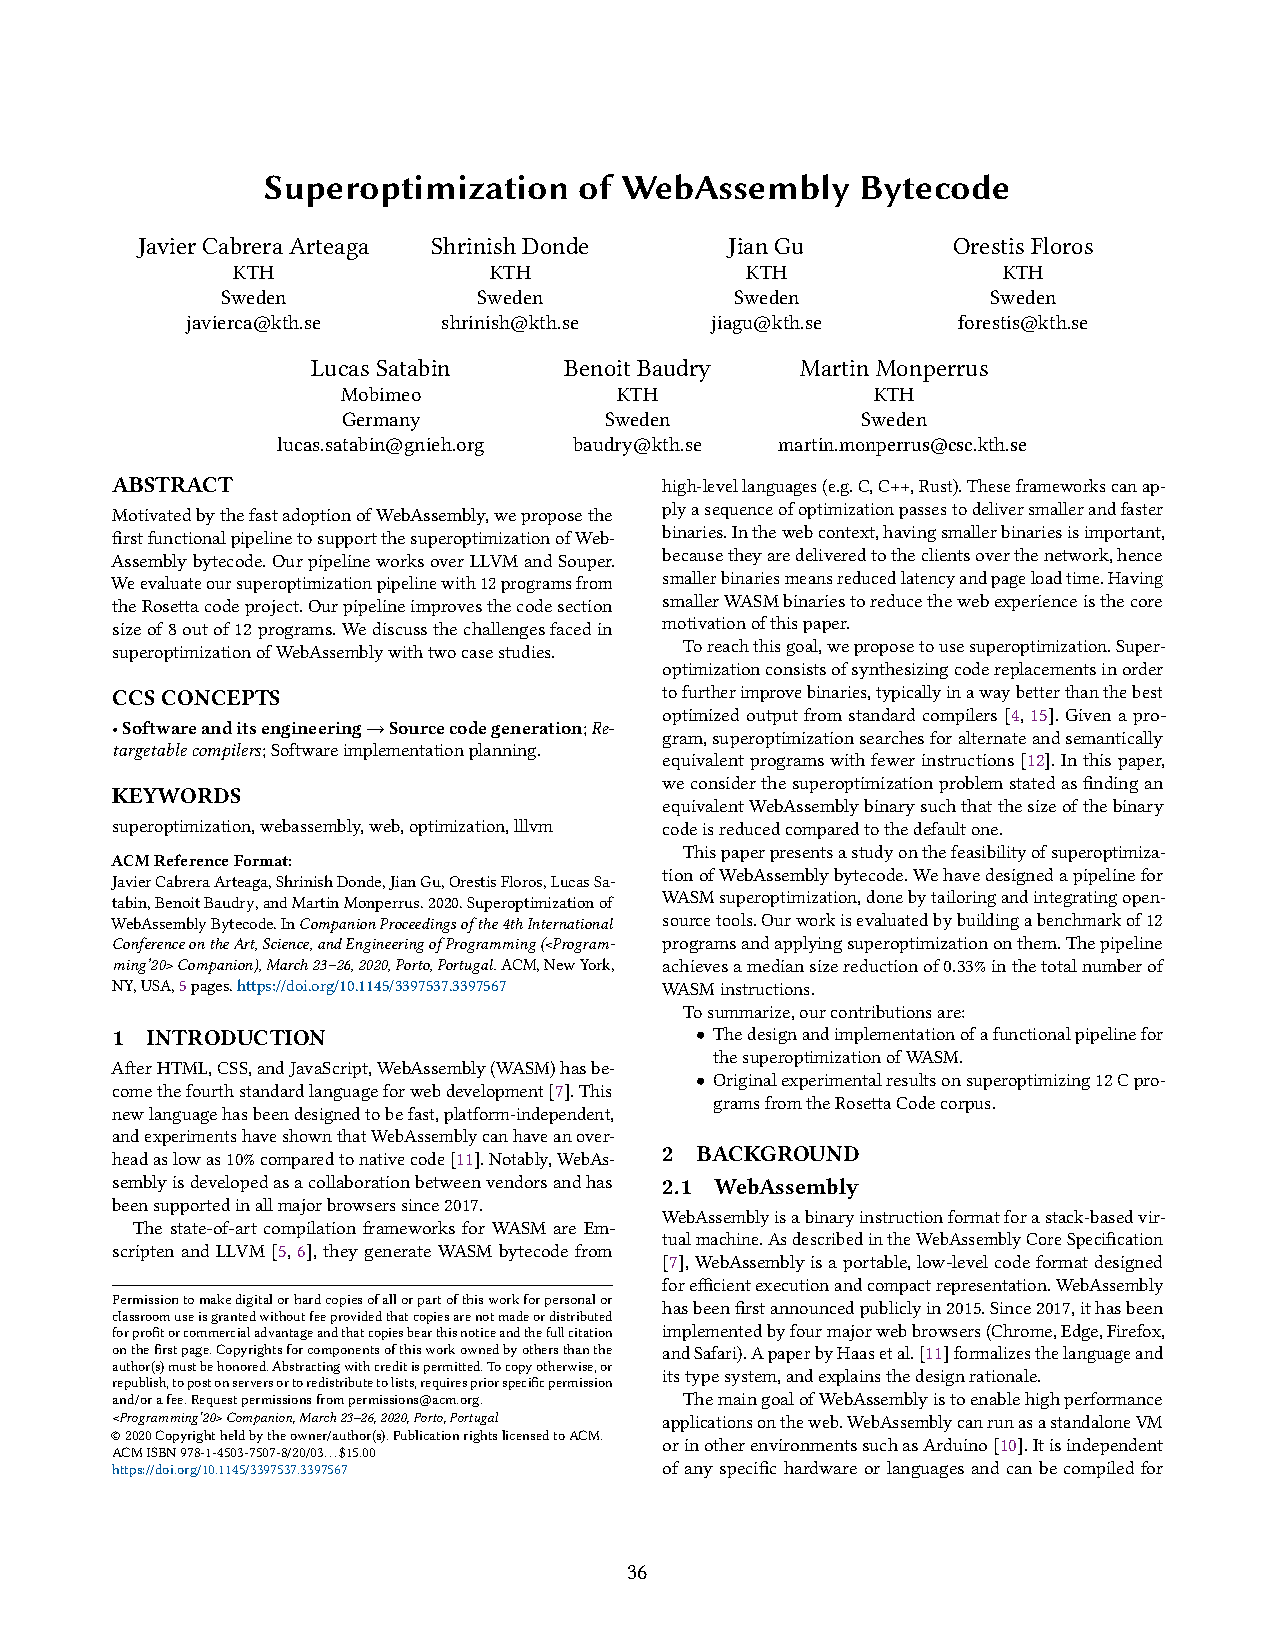
\includepdf[pages=1-5]{papers/souper.pdf}} % 
    {} %

% Add paper here
\chapter{CROW: Code Diversification for WebAssembly}

\textbf{Javier Cabrera-Arteaga}, Orestis Floros, Oscar Vera-Pérez, Benoit Baudry, Martin Monperrus\\
\emph{NDSS 2021, MADWeb}\\

\ifthenelse{\equal{\ADDCONTRIB}{True}}%
    {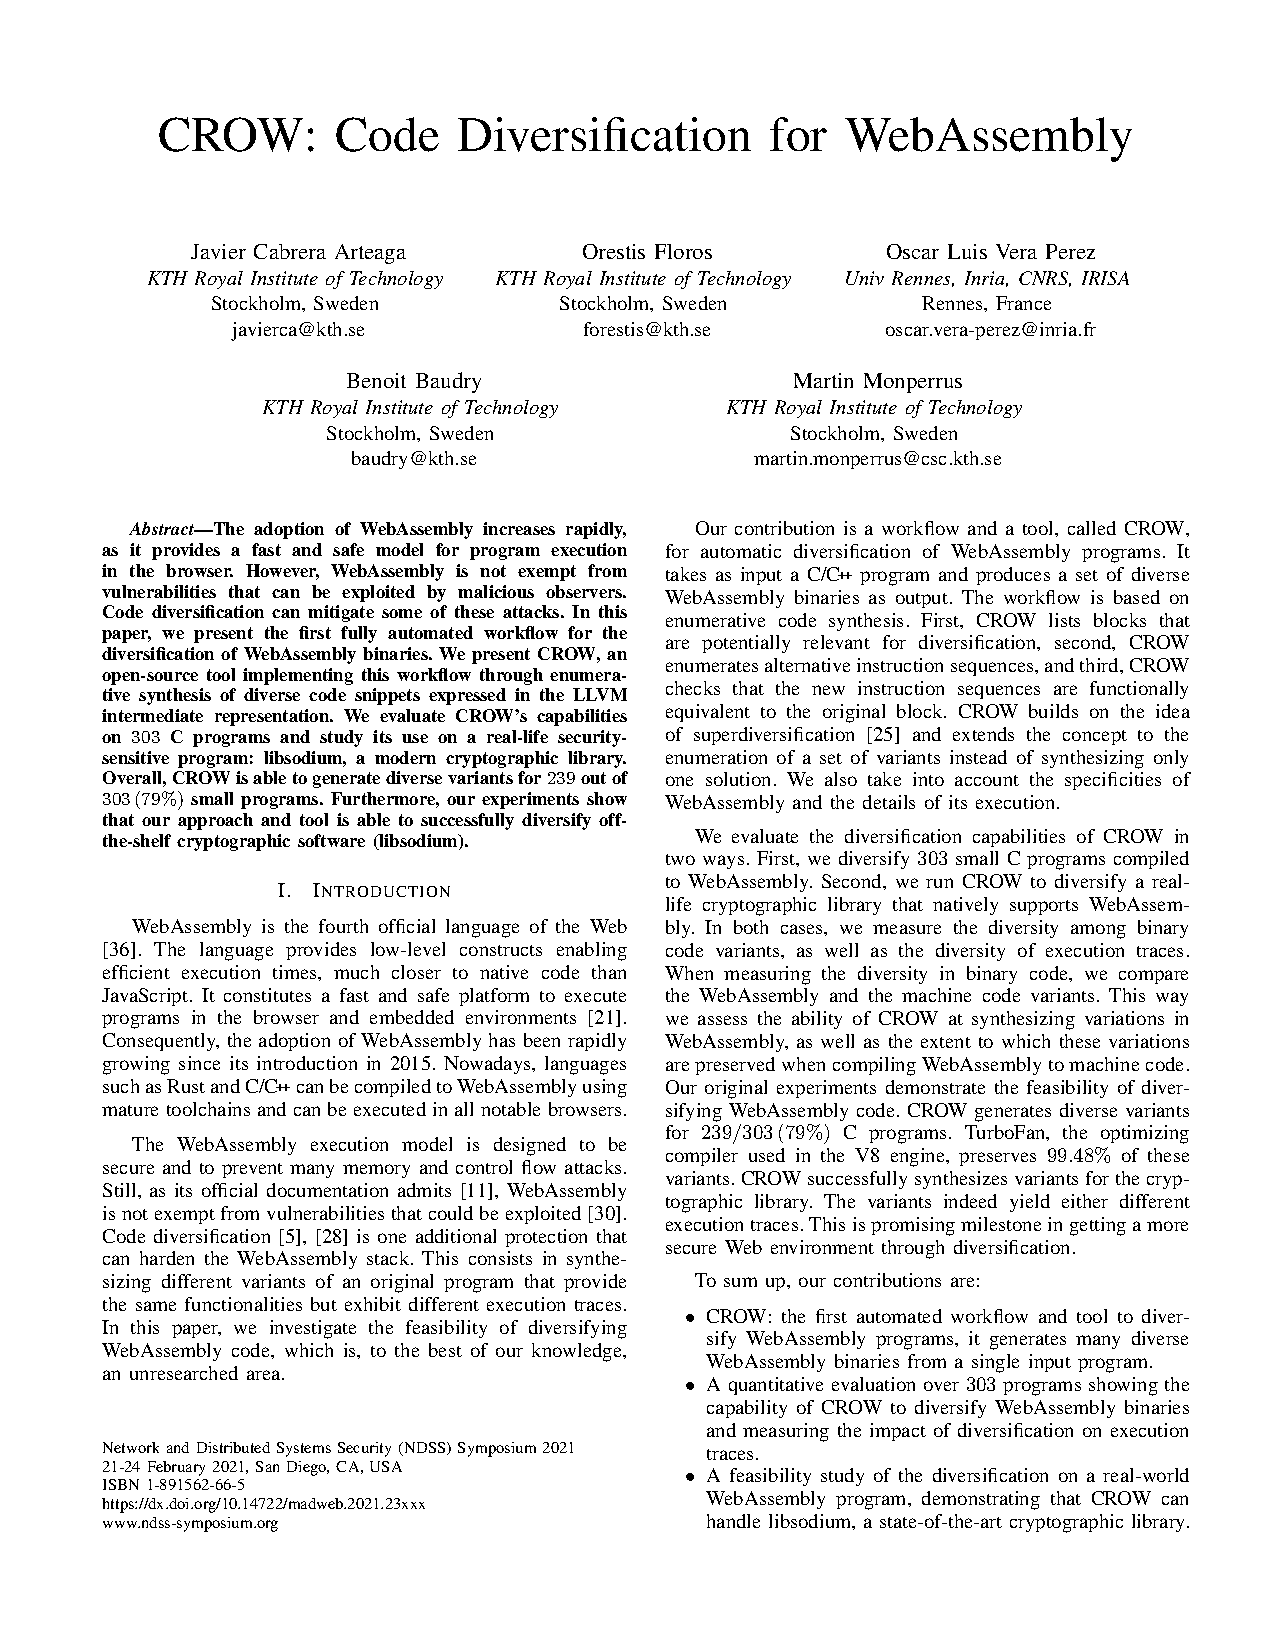
\includepdf[pages=1-12]{papers/crow.pdf}} %
    {} % 
    
\chapter{Multi-Variant Execution at the Edge}

\textbf{Javier Cabrera-Arteaga}, Pierre Laperdrix, Martin Monperrus, Benoit Baudry\\
\emph{Under review}\\

\ifthenelse{\equal{\ADDCONTRIB}{True}}%
    {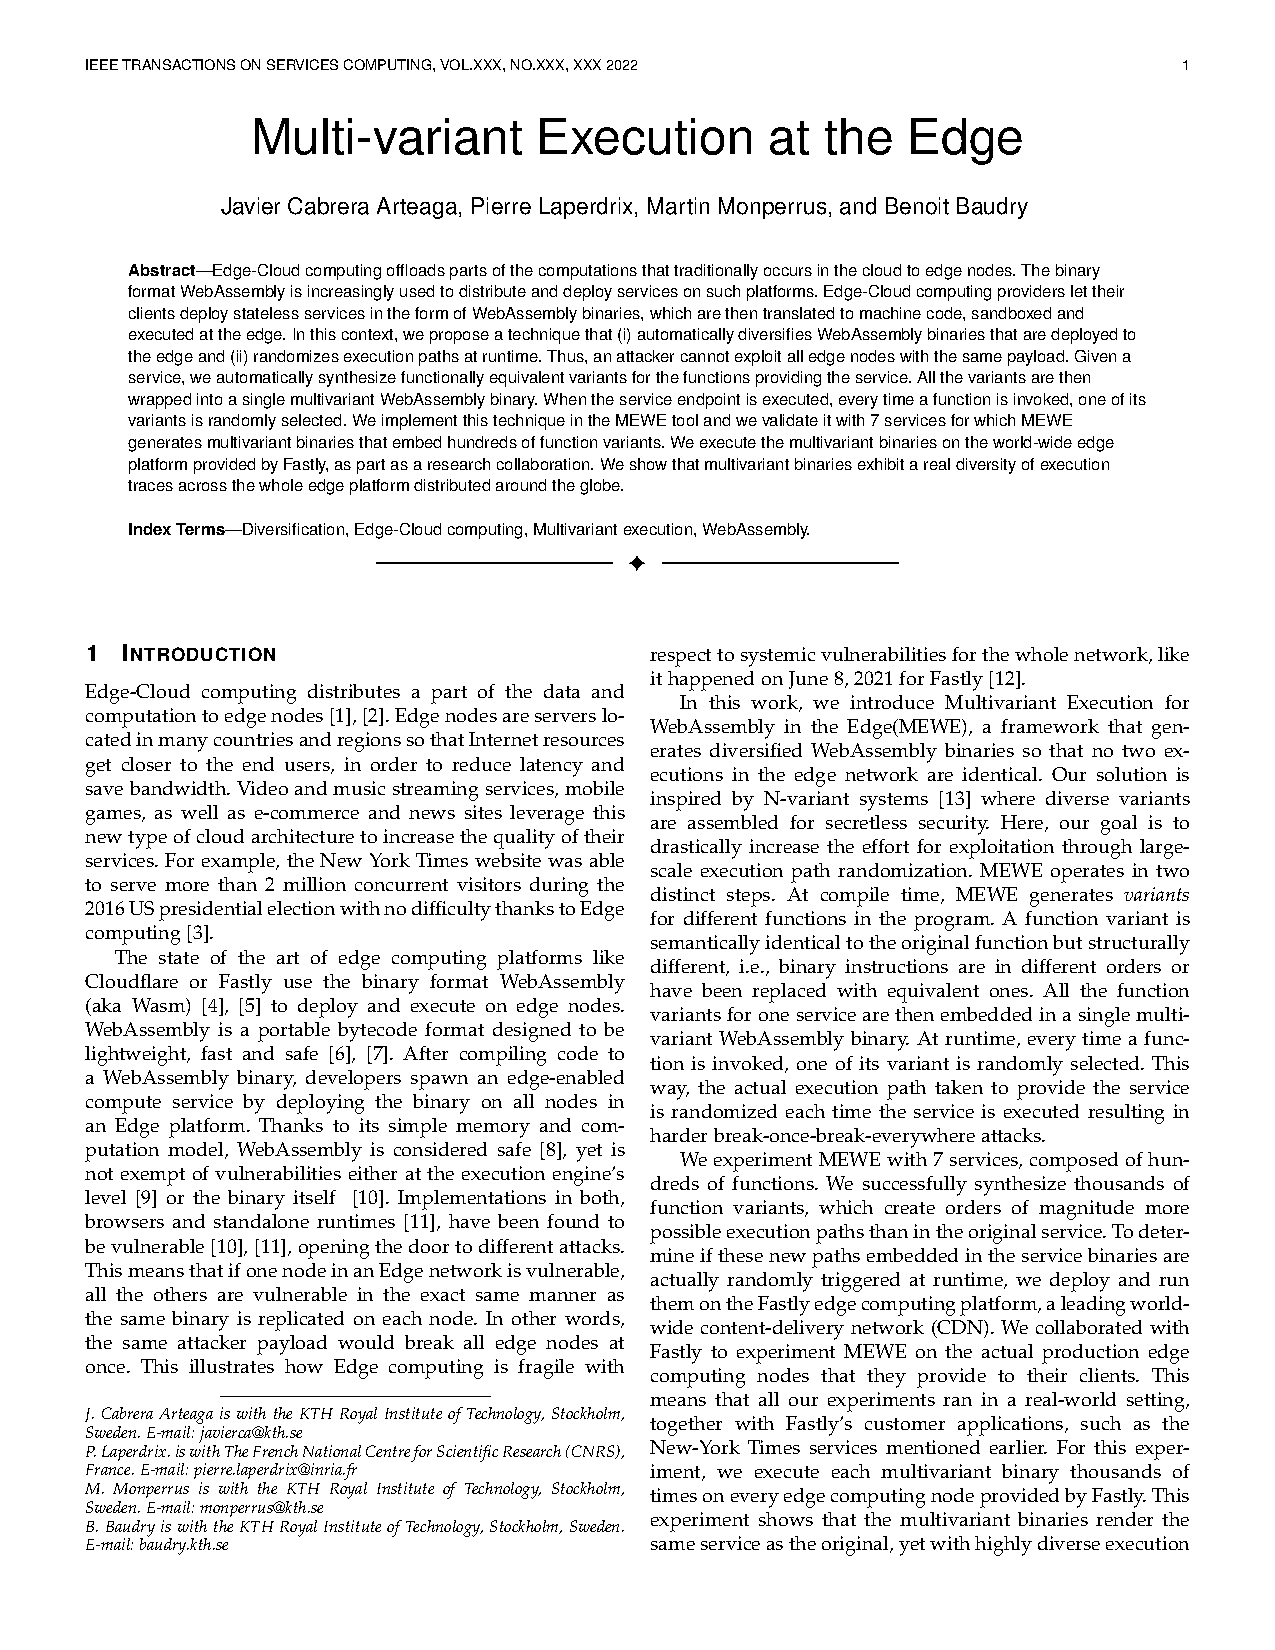
\includepdf[pages=1-12]{papers/mewe2.pdf}} %
    {} %
    
\chapter{Scalable Comparison of JavaScript V8 Bytecode Traces}

\textbf{Javier Cabrera-Arteaga}, Martin Monperrus, Benoit Baudry\\
\emph{SPLASH 2019, VMIL}\\


\ifthenelse{\equal{\ADDCONTRIB}{True}}%
    {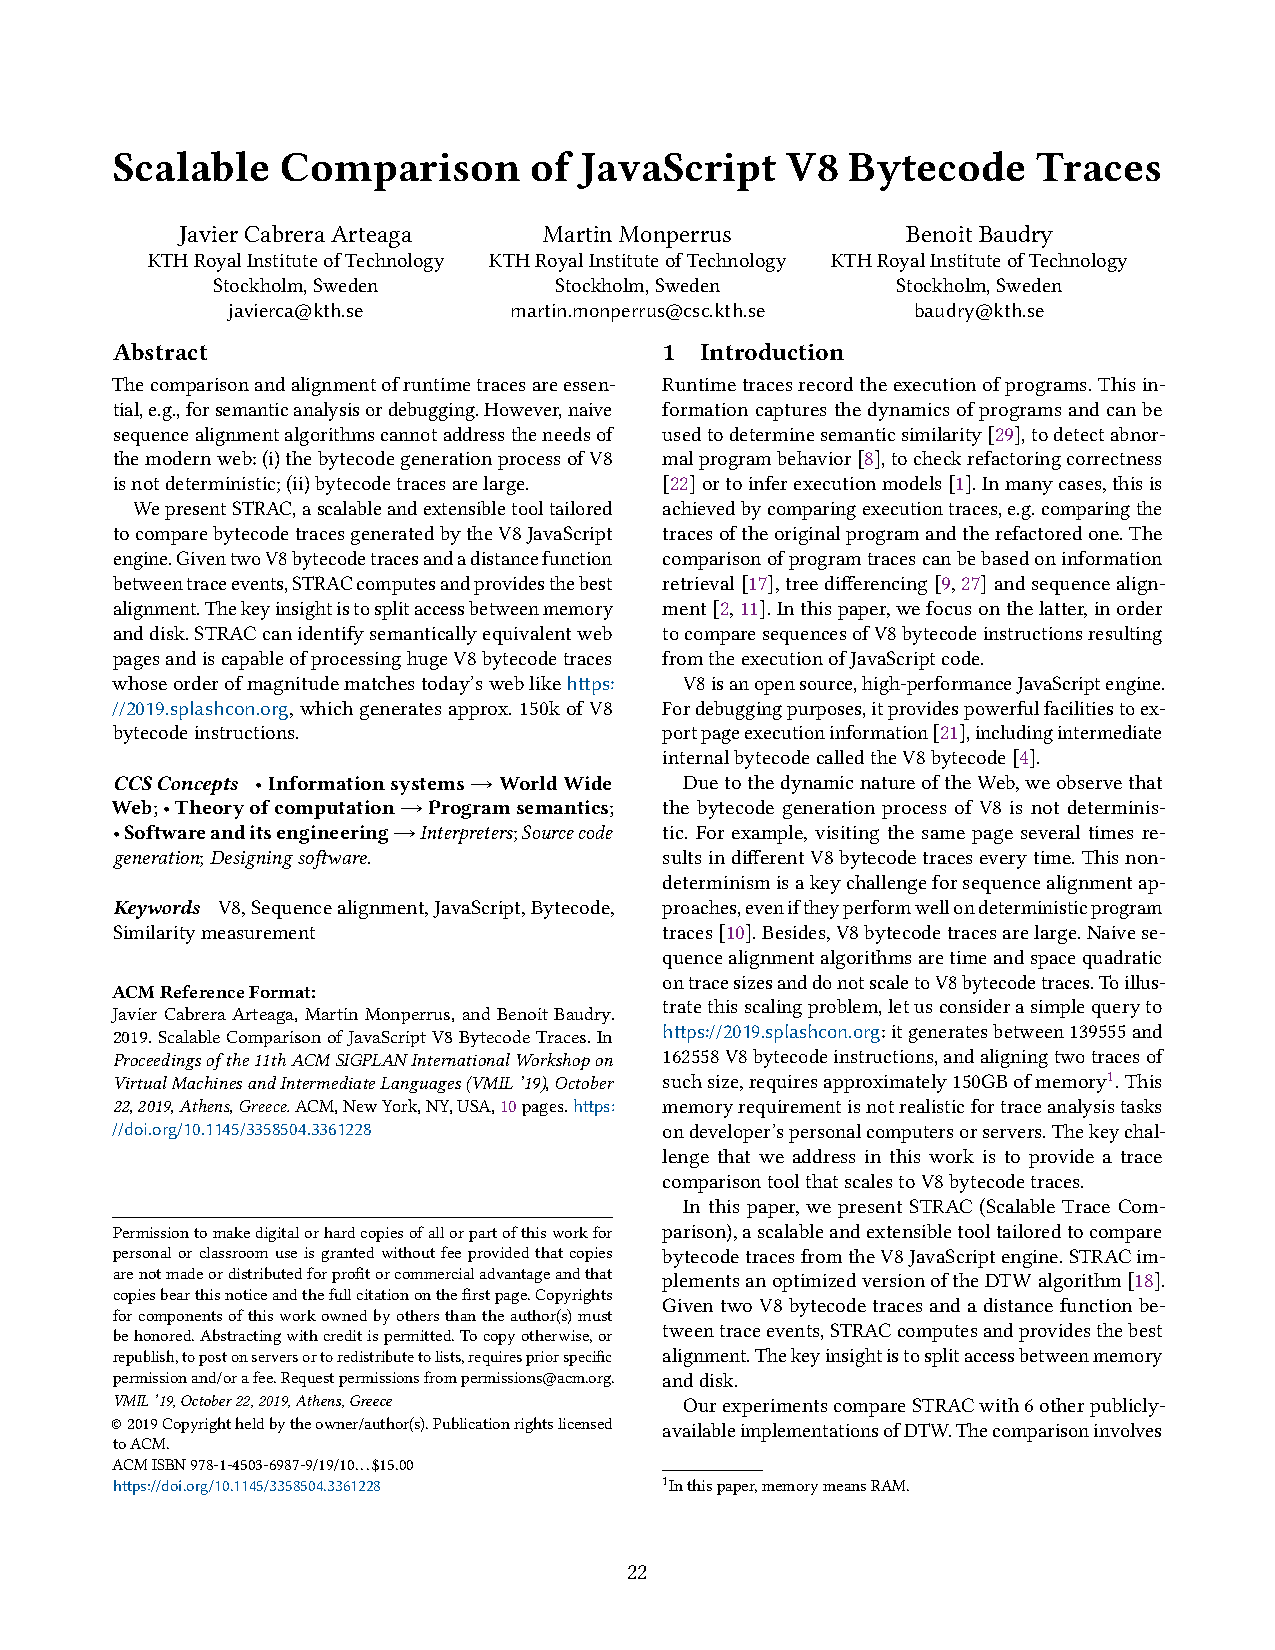
\includepdf[pages=1-10]{papers/STRAC.pdf}} %
    {} %
    

\printindex 

\end{document}
\endinput

